\documentclass[12pt]{report}

\usepackage{tamuconfig}

% Most of the packages that set the default settings
% for the document have moved to the style file
% tamuconfig.sty.

%These next lines change the font. Fixes for certain
%fonts will be implemented in a future release.

%Comment this line if you do not wish to use Times
%New Roman. The font used will then be the LaTeX
%default of Computer Modern.
\usepackage{times}
%\usepackage{cmbright}
\usepackage[T1]{fontenc}

%This package allows for the use of graphics in the
%document.
\usepackage{amsmath, amsthm, amssymb, amsfonts, booktabs, graphicx, float, esint, subcaption, xspace, xcolor}

\usepackage{stix,stmaryrd}
\usepackage{hyperref}

%If you have JPEG format images, add .jpg as an
%allowed file extension below. Same for Bitmaps (.bmp).
\DeclareGraphicsExtensions{.png}

%It is best practice to keep all your pictures in
%one folder inside the main directory in which your
%TeX file is kept. Here the folder is named "graphic."
%Replace the name here with your folder's name, if needed.
%The period is needed due to relative referencing.
\graphicspath{ {./graphic/} }

%%%%%%%%%%%%%%%%%%%%%%%%%%%%%%%%%%%%%%%%%%%%%%%%%%%%%%%%%
%Please place all your personal packages here. Check to
%see if the packages you wish to use are not already
%declared above. Placing all your personal packages
%here allows me to determine if there are any package
%issues in compilation, as well as any conflicts
%that may arise by the order of loading.
%--Sean Zachary Roberson
%%%%%%%%%%%%%%%%%%%%%%%%%%%%%%%%%%%%%%%%%%%%%%%%%%%%%%%%%
%%%%%%%%%%%%%%%%%%%%%%%%%%%%%%%%%%%%%%%%%%%%%%%%%%%%%%%%%
%Begin student defined packages.
%%%%%%%%%%%%%%%%%%%%%%%%%%%%%%%%%%%%%%%%%%%%%%%%%%%%%%%%%


\setlength{\abovedisplayskip}{0pt}
\setlength{\belowdisplayskip}{0pt}
\setlength{\abovedisplayshortskip}{0pt}
\setlength{\belowdisplayshortskip}{0pt}

\newcommand{\vr}{\vec{r}}
\newcommand{\vp}{\vec{p}}
\newcommand{\vOmega}{\vec{\Omega}}
\newcommand{\vJ}{\vec{J}}
\newcommand{\vO}{\vec{\Omega}}
\newcommand{\bra}{\left\langle}
\newcommand{\ket}{\right\rangle}
\newcommand{\sbra}{\left[}
\newcommand{\sket}{\right]}
\renewcommand{\div}{\vec{\nabla} \cdot}
\newcommand{\grad}{\vec{\nabla}}
\newcommand{\vbeta}{\vec{\beta} }
\newcommand{\pdx}{\frac{\partial}{\partial x}}
\newcommand{\pdy}{\frac{\partial}{\partial y}}
\newcommand{\pdz}{\frac{\partial}{\partial z}}
\newcommand{\intrrr}{\int d^3 r \,}
\newcommand{\intrr}{\int d^2 r \,}
\newcommand{\dEdphi}{\partial_\phi E }
\newcommand{\dEdp}{\partial_p E }
\newcommand{\dBdphi}{\partial_\phi B }
\newcommand{\dBdp}{B }
\newcommand{\adj}{\phi^\dag}
\newcommand{\vefadj}{\varphi^\dag}
\newcommand{\surf}{\int_{\partial V}}
\newcommand{\domain}{V}
\newcommand{\bound}{\partial V}
\newcommand{\vn}{\vec{n}}
\newcommand{\Edd}{\mathbb{E}}
\newcommand{\BEdd}{B}
\newcommand{\sigt}{\sigma_t}
\newcommand{\sigs}{\sigma_s}
\newcommand{\siga}{\sigma_a}
\newcommand{\isigt}{\sigma_t^{-1}}
\newcommand{\isigtp}{\sigma_{t,p}^{-1}}
% why \newcommand{\angSource}{q_\Omega}
\newcommand{\angSource}{q}
\newcommand{\scalSource}{q}
\newcommand{\angResp}{q^\dag}
\newcommand{\scalResp}{q^\dag}
\newcommand{\qoi}{{\it QoI}\xspace}


\newcommand{\comment}[2]{\marginpar{\textcolor{#2}{$\star$}}\textcolor{#2}{#1}\newline}

%-----------------------------------------------------------
%-----------------------------------------------------------
\usepackage{ifthen}
\newboolean{draftversion}
\setboolean{draftversion}{true}
%-----------------------------------------------------------
%----------------------------------------------------------

\ifthenelse{\boolean{draftversion}}
{
\newcommand{\iwh}[1]{\comment{#1}{red}}
\newcommand{\jcr}[1]{\comment{#1}{blue}}
\newcommand{\todo}[1]{\comment{#1}{purple}}
}
{
\newcommand{\iwh}[1]{\phantom{a}}
\newcommand{\jcr}[1]{\phantom{a}}
\newcommand{\todo}[1]{\phantom{a}}
}
\newcommand{\tcr}[1]{\comment{#1}{red}}

%%%%%%%%%%%%%%%%%%%%%%%%%%%%%%%%%%%%%%%%%%%%%%%%%%%%%%%%%
%End student defined packages.
%%%%%%%%%%%%%%%%%%%%%%%%%%%%%%%%%%%%%%%%%%%%%%%%%%%%%%%%%

% End preamble. Document begins below.

\begin{document}

%The title of your document goes here.
%Spacing may need to be adjusted if your title is long
%and pushes the copyright off the page.
\renewcommand{\tamumanuscripttitle}{Adjoint-based sensitivity for radiation transport using an Eddington tensor formulation}

%Type only Thesis, Dissertation, or Record of Study.
\renewcommand{\tamupapertype}{Thesis}

%Your full name goes here, as it is in university records. Check your student record on Howdy if there is any mismatch.
\renewcommand{\tamufullname}{Ian Halvic}

%The degree title goes here. See the OGAPS site for more info.
\renewcommand{\tamudegree}{Master of Science}
\renewcommand{\tamuchairone}{Professor Jean Ragusa}


% Uncomment out the next line if you have co-chairs.  You will also need to edit the titlepage.tex file.
%\newcommand{\tamuchairtwo}{Additional Chair Name}
\renewcommand{\tamumemberone}{Professor Marvin Adams}
\newcommand{\tamumembertwo}{Professor Bojan Popov}
\renewcommand{\tamudepthead}{Professor Yassin Hassan}

%Type only May, August, or December.
\renewcommand{\tamugradmonth}{January}
\renewcommand{\tamugradyear}{2017}
%Your department name goes here.
\renewcommand{\tamudepartment}{Nuclear Engineering}


%%%%%%%%%%%%%%%%%%%%%%%%%%%%%%%%%%%%%%%%%%%%%%%%%%%
%
%  New template code for TAMU Theses and Dissertations starting Fall 2016.  
%
%
%  Author: Sean Zachary Roberson
%  Version 3.17.06
%  Last Updated: 6/15/2017
%
%%%%%%%%%%%%%%%%%%%%%%%%%%%%%%%%%%%%%%%%%%%%%%%%%%%

%%%%%%%%%%%%%%%%%%%%%%%%%%%%%% 
%% TITLE PAGE
%% The values get updated automatically.  Please do not make changes to this file other than adding/deleting committee members where necessary.
%%%%%%%%%%%%%%%%%%%%%%%%%%%%%%

\providecommand{\tabularnewline}{\\}



\begin{titlepage}
\begin{center}
\MakeUppercase{\tamumanuscripttitle}
\vspace{4em}

A \tamupapertype

by

\MakeUppercase{\tamufullname}

\vspace{4em}

\begin{singlespace}

Submitted to the Office of Graduate and Professional Studies of \\
Texas A\&M University \\

in partial fulfillment of the requirements for the degree of \\
\end{singlespace}

\MakeUppercase{\tamudegree}
\par\end{center}
\vspace{2em}
\begin{singlespace}
\begin{tabular}{ll}
 & \tabularnewline
& \cr
% If you have Co-Chairs comment out the 'Chair of Committee' line below and uncomment the 'Co-Chairs of Committee' line.
Chair of Committee, & \tamuchairone\tabularnewline
%Co-Chairs of Committee, & \tamuchairone\tabularnewline & \tamuchairtwo\tabularnewline
Committee Members, & \tamumemberone\tabularnewline
 & \tamumembertwo\tabularnewline
% & \tamumemberthree\tabularnewline
Head of Department, & \tamudepthead\tabularnewline

\end{tabular}
\end{singlespace}
\vspace{3em}

\begin{center}
\tamugradmonth \hspace{2pt} \tamugradyear

\vspace{3em}

Major Subject: \tamudepartment \par
\vspace{3em}
Copyright \tamugradyear \hspace{.5em}\tamufullname 
\par\end{center}
\end{titlepage}
\pagebreak{}




 % This is simply a file that formats and adds your titlepage, please do not edit this unless you have a specific need. .
%%%%%%%%%%%%%%%%%%%%%%%%%%%%%%%%%%%%%%%%%%%%%%%%%%%
%%%%%%%%%%%%%%%%%%%%%%%%%%%%%%%%%%%%%%%%%%%%%%%%%%%%%%%%%%%%%%%%%%%%%
%%                           ABSTRACT 
%%%%%%%%%%%%%%%%%%%%%%%%%%%%%%%%%%%%%%%%%%%%%%%%%%%%%%%%%%%%%%%%%%%%%

\chapter*{ABSTRACT}
\addcontentsline{toc}{chapter}{ABSTRACT} % Needs to be set to part, so the TOC doesnt add 'CHAPTER ' prefix in the TOC.

\pagestyle{plain} % No headers, just page numbers
\pagenumbering{roman} % Roman numerals
\setcounter{page}{2}

\todo{I need to loop back to this}
Adjoint methods can provide a first-order approximation of the response a physical system due to a perturbation in the system's parameters. However, when applying the method to a time dependent transport, memory costs can quickly become a concern, and a fully angular dependent flux must be stored at each timestep. Here, a lower-order Variable Eddington Tensor formulation of the transport equation is considered to remove the angular dependence of the stored solution and reduce memory costs. Indeed, given the Eddington tensor, the Eddington tensor approach yields the same answer as the full transport solution.

In the case of perturbations, one may make some simplifying assumption regarding the Eddington tensor: for instance, keep it unperturbed or assuming a functional variation of the Eddington tensor over the input parameter space. An unperturbed Eddington assumption may introduce error in the sensitivity calculation. A simple linear interpolation scheme for the Eddington over the uncertain parameter range is devised for use in certain scenarios, at the cost of requiring a few additional forward Sn-solves to parameterize the Eddington tensor. Results highlighting the approach are presented. An alternate formulation using an Eddington tensor derived from the adjoint transport is also presented, and shows promise in particular scenarios. Comparison of the derived Eddington methods and transport methods is done using slab geometry test cases.


 

\pagebreak{}

%%%%%%%%%%%%%%%%%%%%%%%%%%%%%%%%%%%%%%%%%%%%%%%%%%%%%%%%%%%%%%%%%%%%%%
%%                           DEDICATION
%%%%%%%%%%%%%%%%%%%%%%%%%%%%%%%%%%%%%%%%%%%%%%%%%%%%%%%%%%%%%%%%%%%%%
\chapter*{DEDICATION}
\addcontentsline{toc}{chapter}{DEDICATION}  % Needs to be set to part, so the TOC doesnt add 'CHAPTER ' prefix in the TOC.



\begin{center}
\vspace*{\fill}
\todo{Add Dedications Here}
\vspace*{\fill}
\end{center}

\pagebreak{}

%%%%%%%%%%%%%%%%%%%%%%%%%%%%%%%%%%%%%%%%%%%%%%%%%%%%%%%%%%%%%%%%%%%%%%
%%                           ACKNOWLEDGMENTS
%%%%%%%%%%%%%%%%%%%%%%%%%%%%%%%%%%%%%%%%%%%%%%%%%%%%%%%%%%%%%%%%%%%%%
\chapter*{ACKNOWLEDGMENTS}
\addcontentsline{toc}{chapter}{ACKNOWLEDGMENTS}  % Needs to be set to part, so the TOC doesnt add 'CHAPTER ' prefix in the TOC.
I would like to thank my advisor Professor Jean Ragusa for his invaluable help on this work and other academic endeavors. 



\pagebreak{}
%%%%%%%%%%%%%%%%%%%%%%%%%%%%%%%%%%%%%%%%%%%%%%%%%%%%%%%%%%%%%%%%%%%%%%
%%             CONTRIBUTORS AND FUNDING SOURCES
%%%%%%%%%%%%%%%%%%%%%%%%%%%%%%%%%%%%%%%%%%%%%%%%%%%%%%%%%%%%%%%%%%%%%
\chapter*{CONTRIBUTORS AND FUNDING SOURCES}
\addcontentsline{toc}{chapter}{CONTRIBUTORS AND FUNDING SOURCES}  % Needs to be set to part, so the TOC doesn't add 'CHAPTER ' prefix in the TOC.


%This section is taken directly from the MS Word templates.

%Old version below.

%All theses and dissertations must include a contributors and funding sources section. In this section, name all members of the dissertation committee, and any collaboration with others in carrying out your thesis or dissertation research. Your independent contributions must be made clear.
%
%If financial support from the university or any other source was gained to conduct your thesis or dissertation research and compilation, it must be listed in this section. If you completed all work independently without outside financial support, indicate this here.
%\textit{(Sample Wording)}
%
%This work was supported by a dissertation committee consisting of Professor XXX [advisor – also note if co-advisor] and XXXX of the Department of [Home Department] and Professor(s) XXXX of the Department of [Outside Department].
% 
%The data analyzed for Chapter III was provided by Professor XXXX. The analyses depicted in Chapter IV were conducted in part by Rebecca Jones of the Department of Biostatistics and were published in (year) in an article listed in the Biographical Sketch. 
%
%All other work conducted for the dissertation was completed by the student independently.
%
%\noindent \textit{(or)}
%
%This work was supervised by a dissertation committee consisting of Professor XXXX [advisor – also note if co-advisor] and Professor(s) XXXX of the Department of [Home Department] and Professor(s) XXXX of [Outside Department]. All work for the dissertation was completed independently by the student.
%
%\noindent \textit{(or)}
%
%Graduate study was supported by a fellowship from Texas A\&M University and a dissertation research fellowship from XXX Foundation.

\subsection*{Contributors}
This work was supported by a thesis (or) dissertation committee consisting of Professor Jean Ragusa and Professor Marvin Adams of the Department of Nuclear Engineering and Professor Bojan Popov of the Department of Mathematics.


All other work conducted for the thesis (or) dissertation was completed by the student independently.
\subsection*{Funding Sources}
Graduate study was supported by a fellowship from Texas A\&M University and a dissertation research fellowship from XXX Foundation. 
\pagebreak{}
%%%%%%%%%%%%%%%%%%%%%%%%%%%%%%%%%%%%%%%%%%%%%%%%%%%%%%%%%%%%%%%%%%%%%%
%%                           NOMENCLATURE
%%%%%%%%%%%%%%%%%%%%%%%%%%%%%%%%%%%%%%%%%%%%%%%%%%%%%%%%%%%%%%%%%%%%%

\chapter*{NOMENCLATURE}
\addcontentsline{toc}{chapter}{NOMENCLATURE}  % Needs to be set to part, so the TOC doesnt add 'CHAPTER ' prefix in the TOC.

%A note about aligning: These entries will align
%themselves according to the ampersand (&).
%No extra spaces are needed, as seen in some of
%the entries below.

%Example of the longtable environment.
\hspace*{-1.25in}
\vspace{12pt}
\begin{spacing}{1.0}
	\begin{longtable}[htbp]{@{}p{0.35\textwidth} p{0.62\textwidth}@{}}
	   % \begin{tabular}{@{}p{0.33\textwidth} p{0.62\textwidth}@{}}
		VET 		& Variable Eddington Tensor\\	[2ex]
		aVET 		& Adjoint Variable Eddington Tensor\\	[2ex]
		SN 			& Discrete Ordinate Method\\	[2ex]
	   % \end{tabular}%
	\end{longtable}
\end{spacing}

\pagebreak{}

%%%%%%%%%%%%%%%%%%%%%%%%%%%%%%%%%%%%%%%%%%%%%%%%%%%
%
%  New template code for TAMU Theses and Dissertations starting Fall 2016.  
%
%
%  Author: Sean Zachary Roberson
%  Version 3.17.06
%  Last Updated: 6/15/2017
%
%%%%%%%%%%%%%%%%%%%%%%%%%%%%%%%%%%%%%%%%%%%%%%%%%%%
%%%%%%%%%%%%%%%%%%%%%%%%%%%%%%%%%%%%%%%%%%%%%%%%%%%%%%%%%%%%%%%%%%%%%%
%%       TABLE OF CONTENTS
%%%%%%%%%%%%%%%%%%%%%%%%%%%%%%%%%%%%%%%%%%%%%%%%%%%%%%%%%%%%%%%%%%%%%
% single-space sections in Table of Contents  - commented in version 1.7
%\renewcommand{\cftsecafterpnum}{\vskip0.5\baselineskip}
%\renewcommand{\cftsubsecafterpnum}{\vskip0.5\baselineskip}
%\renewcommand{\cftsubsubsecafterpnum}{\vskip0.5\baselineskip}
%%%%%%%%%%%%%%%%%%%%%%%%%%%%%%%%%%%%%%%%%%%%%%%%%%%

\phantomsection
\addcontentsline{toc}{chapter}{TABLE OF CONTENTS}  

\begin{singlespace}
\renewcommand\contentsname{\normalfont} {\centerline{TABLE OF CONTENTS}}

\setcounter{tocdepth}{4} % This puts \subsubsection[]{×} in your List of Tables.  The default is 3.


%%%%%%%%%%%%%  Adds Page above the page number in TOC
\setlength{\cftaftertoctitleskip}{1em}
\renewcommand{\cftaftertoctitle}{%
\hfill{\normalfont {Page}\par}}


\tableofcontents

%\addtocontents{toc}{\protect\afterpage{~\hfill\normalfont{Page}\par\medskip}}
\end{singlespace}

\pagebreak{}

%%%%%%%%%%%%%%%%%%%%%%%%%%%%%%%%%%%%%%%%%%%%%%%%%%%%%%%%%%%%%%%%%%%%%%
%%                           LIST OF FIGURES
%%%%%%%%%%%%%%%%%%%%%%%%%%%%%%%%%%%%%%%%%%%%%%%%%%%%%%%%%%%%%%%%%%%%%

\phantomsection
\addcontentsline{toc}{chapter}{LIST OF FIGURES}  

\renewcommand{\cftloftitlefont}{\center\normalfont\MakeUppercase}

\setlength{\cftbeforeloftitleskip}{-12pt} %% Positions the LOF title vertically to match the chapter titles
\renewcommand{\cftafterloftitleskip}{12pt}


\renewcommand{\cftafterloftitle}{%
\\[4em]\mbox{}\hspace{2pt}FIGURE\hfill{\normalfont Page}\vskip\baselineskip}

\begingroup


\begin{center}
\begin{singlespace}
%% These values make the lof table entries appear double spaced between.
\setlength{\cftbeforechapskip}{0.4cm}
\setlength{\cftbeforesecskip}{0.30cm}
\setlength{\cftbeforesubsecskip}{0.30cm}
\setlength{\cftbeforefigskip}{0.4cm}
\setlength{\cftbeforetabskip}{0.4cm}

% Provided by Andy Philips.
% needed to make chapter gaps look no different than sections:
% \addtocontents{lof}{\protect\renewcommand*\protect\addvspace[1]{}}

% Philips' document had 30 figures. Is there a maximum number of figures
% that changes the spacing to non-uniform, i.e., not double-spaced
% between all entries?

\listoffigures

\end{singlespace}
\end{center}

\pagebreak{}


%%%%%%%%%%%%%%%%%%%%%%%%%%%%%%%%%%%%%%%%%%%%%%%%%%%%%%%%%%%%%%%%%%%%%%
%%                           LIST OF TABLES
%%%%%%%%%%%%%%%%%%%%%%%%%%%%%%%%%%%%%%%%%%%%%%%%%%%%%%%%%%%%%%%%%%%%%%
%
\phantomsection
\addcontentsline{toc}{chapter}{LIST OF TABLES}  

\renewcommand{\cftlottitlefont}{\center\normalfont\MakeUppercase}

\setlength{\cftbeforelottitleskip}{-12pt} %% Positions the LOT title vertically to match the chapter titles

%Note that the similar parameter in the LOF is 12pt; this
%is intentional to make the spacing between the headers
%and the first entry look consistent.
\renewcommand{\cftafterlottitleskip}{1pt}


\renewcommand{\cftafterlottitle}{%
\\[4em]\mbox{}\hspace{2pt}TABLE\hfill{\normalfont Page}\vskip\baselineskip}

\begin{center}
\begin{singlespace}

%% These values make the lot table entries appear double spaced between.
\setlength{\cftbeforechapskip}{0.4cm}
\setlength{\cftbeforesecskip}{0.30cm}
\setlength{\cftbeforesubsecskip}{0.30cm}
\setlength{\cftbeforefigskip}{0.4cm}
\setlength{\cftbeforetabskip}{0.4cm}

\listoftables 

\end{singlespace}
\end{center}
\endgroup
\pagebreak{}  % Need this for the pagenumbering to be correct.   % This is simply a file that formats and adds your toc, lof, and lot, please do not edit this unless you have a specific need.

%%%%%%%%%%%%%%%%%%%%%%%%%%%%%%%%%%%%%%%%%%%%%%%%%%%%%%%%%%%%%%%%%%%%%%
%%                           SECTION I
%%%%%%%%%%%%%%%%%%%%%%%%%%%%%%%%%%%%%%%%%%%%%%%%%%%%%%%%%%%%%%%%%%%%%


\pagestyle{plain} % No headers, just page numbers
\pagenumbering{arabic} % Arabic numerals
\setcounter{page}{1}


\chapter{\uppercase {Introduction}}

%%%%%%%%%%%%%%%%%%%%%%%%%%%%%%%%%%%%%%%%%%%%%%%%%%%%%%%%%%%%%%%%%%%%%%%%%%%%%%%%%%%%%%%%%%%%%%%%%%%%
\section{Introduction}
%%%%%%%%%%%%%%%%%%%%%%%%%%%%%%%%%%%%%%%%%%%%%%%%%%%%%%%%%%%%%%%%%%%%%%%%%%%%%%%%%%%%%%%%%%%%%%%%%%%%

Computational simulations have become important tools for engineers and scientists across a wide array of disciplines. These simulations allow for researchers to examine significantly complex and long life systems in a way that is frequently more economical in both time and money than construction of the real world system, if even feasible. An important step in creating one of these methods is confirmation that the results can be trusted to reasonably approximate the real life scenario. This can be accomplished using three process outlined by the National Research Council \cite{NRCVVUQ}


\begin{itemize}
\item Verification - How accurately does the computation solve the underlying equations of the model for the quantities of interest?
\item Validation - How accurately does the model represent reality for the quantities of interest?
\item Uncertainty Quantification (UQ) -  How do the various sources of error and uncertainty feed into uncertainty in the model-based prediction of the quantity of interest?
\end{itemize}


Adjoint methods are particularly useful for UQ. In general, adjoint methods provide a mechanism for computing quantities of interest (\qoi) and sensitivity coefficients and, more generally, for propagating uncertainty and error in the system variables to the error in the desired quantity of interest. They accomplish this in a particularly economical way, requiring only two full system solves (one forward and one adjoint solve) in steady state in order to determine first-order sensitivity coefficients for any combination of sources of uncertainty, as opposed to performing multiple forward system solves to determine
the sensitivity due to each individual uncertain parameter.

Using operator notation to denote the forward and adjoint (linear\footnote{The forward problem may be nonlinear, i.e., using $A(u)$, but the adjoint problem is linear, evaluated at $u$ if the forward problem is nonlinear, i.e., using $A^\dag(u)$}) problems, $Au=q$ and $A^\dag u^\dag = q^\dag$, respectively, and the bracket notation for inner products over the phase space, it is easy to note that a \qoi can 
obtained using {\it either} the forward solution $u$ folded with the response function of interest (which is also the adjoint source, $q^\dag$) {\it or} the adjoint solution folded with the forward source~:
\[
\qoi = \bra u, q^\dag \ket = \bra u^\dag, q \ket \,.
\]
The sensitivity coefficient due to parameter $p$ can be obtained using two forward solves
\[
\delta_p \qoi = \frac{\qoi^\prime - \qoi}{\delta p} = \frac{ \bra (u^\prime - u), q^\dag \ket}{p^\prime - p}  \,,
\]
where the superscript $^\prime$ denotes a perturbed value. However, one may employ the unperturbed adjoint solution to obtain
a {\it first-order} estimate of the sensitivity coefficient
\[
\delta_p \qoi = \bra u^\dag, \delta_p q - \delta_p A u \ket \,.
\]
\jcr{since this is the thesis, the above expression should be demonstrated later. I understand that this chapter is only the intro, so you give a rapid overview...}
The subsequent sections will provide additional details and will apply these formulations to neutron transport problems. However, it is already evident that if the forward source $q$ is uncertain and only a few \qoi are requested, it is preferable to employ the adjoint formulation to compute the quantity of interest (one needs only one adjoint solution per response function). Furthermore, the sensitivity of the
\qoi to many uncertain parameters is more advantageously computed using the adjoint.


Adjoint methods are of particular interest for UQ. In general, adjoint methods provide a mechanism for propagating uncertainty and error in the system variables to the error in the desired quantity of interest. Adjoint methods accomplish this in a particularly economical way, sometimes requiring only two differential system solves which can then be used for any combination of sources of error, as opposed to performing an independent solve for each individual error scenario. These adjoint methods have been applied across various complex and time dependent systems. An example of adjoint methods applied to hydrodynamic systems with shocks can be found in Wildey et al. \cite{Wildey}. A more relevant adjoint example to neutron transport occurs in Stripling et al. in the form of reactor burn-up equations \cite{Stripling}.


Application of the adjoint method to time-dependent transport can pose a major technical limitation. In general, the adjoint method applied to radiation transport requires storing six-dimensional data (the forward angular flux) at each time step. When dealing with high resolution in these six dimensions and many time steps, this can potentially require an unreasonable amount of memory for data storage, rendering the method functionally unusable. For the previously mentioned depletion reactor problem of Stripling, this limitation was not existent because a quasi-static approximation was used for the neutron transport equation and only isotopic concentrations were time-dependent. For time-independent radiation problems, only storing the converged scattering moments at defined checkpoints (in burnup) is sufficient to reconstruct the flux solution. If a flux solution is requested outside of the checkpointed burnups, the forward flux can be reconstructed by interpolation \cite{Stripling}.
Using converged scattering source term, a single transport sweep is needed to recover the converged
angular flux. However this method does not extend to time-dependent transport in general because
the primary time-dependent variable, the angular flux, needs to be stored as well. 

A potential solution to the memory requirement for the time-dependent transport adjoint formulation is the use of a quasi-diffusion method to reduce the overall dimensionality of the transport problem, from 6D+time (space, direction, energy, time for transport) to 4D+time (space, energy, time for quasi-diffusion). The method examined in this work is termed  as a ``Variable Eddington Tensor'' formulation and uses the unperturbed forward angular flux to compute the Eddington tensor needed in the quasi-diffusion approach.


%%%%%%%----------------------------------------------------------------------------------------------
\subsection{Steady-state one-group neutron transport equation}
%%%%%%%----------------------------------------------------------------------------------------------
\jcr{I do not understand the numbering. why is this a subsection of the introduction?}

This work will focus on a relatively simple transport equation form, the one-group steady-state transport equation. Examination of the quasi-diffusion's effectiveness in this setting will provide sufficient insight to advantages and shortcomings of the technique when applied to multigroup, time-dependent transport equation. The one-group steady-state transport equation with isotropic scattering for a volume $V$ bounded by its surface $\partial V$ is given below.
\jcr{I think we discussed how VEF would be applied to transient and did some derivations. I think these need to be included somewhere because (1) this is why we decided to look at VEF, and (2) to write the derivation down and not lose it in the future}
\begin{equation}
\label{SS1GTE}
\vO \cdot \grad \psi(\vr,\vO) + \sigt(\vr) \psi(\vr,\vO) = \frac{1}{4 \pi} \sigs(\vr) \phi(\vr) + q(\vr,\vO), \quad \forall \vr \in V
\end{equation}
\begin{equation}
\label{SS1GTE_bc}
\psi(\vr,\vO) = \psi^{\text{inc}}(\vr,\vO) \quad \vr \in \partial V^{-} = \{ \vr \in \partial V, \text{ s.t. }, \vO \cdot \vec{n}(\vr) < 0\}
\end{equation}
The possibly uncertain parameters in this system are: the total and scattering cross sections $\sigt$ and $\sigs$, the volumetric source term $q$, and the incident angular flux on the system given by $\psi^{\text{inc}}$. The unknowns (dependent variables) are the angular flux $\psi(\vr,\vO)$ and the scalar flux $\phi(\vr)$ given by
\[
\phi(\vr) = \int_{4\pi}d\Omega\,\psi(\vr,\vO) \,.
\]
%%%%%%%----------------------------------------------------------------------------------------------
%\subsection{Quantity of interest and their sensitivities}
%%%%%%%----------------------------------------------------------------------------------------------

%----------------------------------------------------------------------------------------------
\subsubsection{Quantity of interest, response function, and inner products}
%----------------------------------------------------------------------------------------------
Frequently, the solution to the transport equation is not the sought after value, but rather some Quantity of Interest (\qoi), a functional that depends on the transport solution. Given $\psi(\vr,\vO)$ the solution of the one-group steady-state transport (Eq.~\eqref{SS1GTE}), a \qoi
defined as
\begin{equation}
\qoi =  \int_V dV \int_{4 \pi} d \vO \,  R(\vr, \vO) \psi(\vr, \vO)
\end{equation}
where $R(\vr, \vO)$ is termed the ``response function'' which is used to characterize the meaning of the desired \qoi. The response function can take on physically defined forms, such as the cross section of a detector; or it may take a form of a mathematical construct, such as $R(\vr, \vO)=1/v$ to return the total number of neutrons present in the system. Another example is to let $R(\vr, \vO)=\sigma \chi(\vr)$ to obtain the total reactor in a portion of the domain ($\chi(\vr)=1$ if $\vr \in$ region of interest, and 0 otherwise). To avoid confusion with the spatial location vector $\vr$, the response function will frequently be expressed as $q^\dag$, the adjoint source, as we have already noted that there is a relationship between the solution, the adjoint solution, and their respective source terms. 

For the sake of brevity in this Thesis, particularly for expressing the \qoi, two volumetric inner products are defined both using $\bra \bullet , \bullet \ket$ notation. These two inner-products are for use with angular and scalar flux respectively. 
\begin{subequations}
\begin{equation}
\bra \psi , \angResp \ket_{V \times \mathcal{S}_2}  = \int_V dV \int_{4 \pi} d \Omega \,  \psi(\vr, \vO)\angResp(\vr, \vO)
\end{equation}
where $\mathcal{S}_2$ denotes the unit sphere.
\begin{equation}
\bra \phi(\vr) ,\angResp \ket_V  = \int_V dV \,  \phi(\vr)\angResp(\vr)
\end{equation}
\end{subequations}
For later use, two additional inner products are also defined as surface integrals over the region boundary $\partial V$. The latter splinting incoming and outgoing surface integrals.
\jcr{did you want to say 'splinting'?}
\begin{subequations}
\begin{equation}
\sbra \psi , g \sket_{\bound \times \mathcal{S}_2}  = \int_{\bound} dS \int_{4 \pi} d \Omega \, \vO \cdot \vn(\vr) \, \psi(\vr, \vO)g(\vr, \vO)
\end{equation}
\begin{equation}
\sbra \psi , g \sket_{\pm}   = \int_{\bound} dS \int_{\vO \cdot \vn \gtrless 0} d\Omega \,  \vO \cdot \vn(\vr) \, \psi(\vr, \vO)g(\vr, \vO)
\end{equation}
\end{subequations}

The inner product subscripts will frequently be dropped when it is unambiguous which one is being used, typically indicated by the presence of an angular-dependent variable, e.g., $\psi$ or an angular-independent variable, e.g., $\phi$. Therefore, with this notation, the quantity of interest can be compactly expressed as shown below.
\begin{equation}
\label{QoIDef}
\qoi = \bra \psi(\vr,\vO), \angResp(\vr,\vO) \ket  = \bra \phi(\vr) , \scalResp(\vr) \ket
\end{equation}
The boundary terms arise from the integration by parts of the streaming terms.
\jcr{what boundary terms? you expression is not complete, you forgot the boundary terms}
\jcr{additionally, I believe you should start demonstrating these relationships. It is fine in the abstract, early introduction, but here we are getting into some details. Imagine another
first-year grad student reading this, they would wonder were these expressions are coming from, espcially if they never heard of adjoint equations}

%----------------------------------------------------------------------------------------------
\subsubsection{Sensitivity Coefficients}
%----------------------------------------------------------------------------------------------
A hurdle in utilizing the transport equation numerically to make real world predictions is that none of the system's parameters ($\sigt$, $\sigs$, $q$, and $\psi^{inc}$) are not known exactly. This error in the system parameters is expected to translate to error in the \qoi value. Ideally, a reasonable error range would be determined for each system parameter and the system simulation would run over a finely discretized parameter space, using the resulting \qoi values to generate an error range for the \qoi. However, this straightforward method tends to be resource-intensive, requiring a complete forward solve of the transport equation for each input error scenario. Adjoint methods offer a way to drastically reduce the number of solves, while generally remaining fairly accurate for small perturbations around base or nominal values of the parameters.

\jcr{we have already talked about this. Here A is in bold font and earlier, it was not. this is not consistent and you must choose one representation and stick with it}
%%%%%%%----------------------------------------------------------------------------------------------
\subsection{Adjoint Sensitivity}
%%%%%%%----------------------------------------------------------------------------------------------

Adjoint operators can provide a useful tool for sensitivity calculations. Using inner product notation $\bra \cdot , \cdot \ket$, consider the system of interest $A \psi = q$. Call this this the forward system, with forward operator $\mathbf{A}$. Consider a test function $\psi^\dag$, the adjoint operator $A^\dag$ is defined such that $\bra \mathbf{A} \psi, \psi^\dag \ket = \bra \psi, A^\dag \psi^\dag \ket $. For differential operators, derivation of $A^\dag$ generally relies on application of the divergence theorem (integration by parts), typically resulting in boundary terms ($BC$). Using the response function of the desired \qoi, the adjoint system can be constructed as $\mathbf{A^\dag} \psi^\dag = q^\dag$, leading to an alternate expression of the \qoi using the adjoint solution $\psi^\dag $.
\begin{equation}
\label{genAdjQoI}
\qoi = \bra \psi, R \ket = \bra q , \psi^\dag \ket + BC
\end{equation} 
From the above, it follows that a first-order approximation to the change in the quantity of interest based on perturbations to the initial system, including perturbation to the forward operator $\delta \mathbf{A}$ and forward source $\delta q$, can be expressed in the form shown in Eq.~\eqref{genAdjSens} \cite{Marchuk}.
\begin{equation}
\label{genAdjSens}
\delta \qoi \approx \bra \delta q - \delta \mathbf{A} \psi , \psi^\dag \ket 
\end{equation}
The advantage of the above expression for $\delta \qoi$ is that two solves, one for the forward and another for the adjoint, can be used to approximate the sensitivity for a variety $\delta \mathbf{A}$ and $\delta q$.
\jcr{in the thesis, you need to go through the algebra for the transport and the VET equations. not here, this is only the proposal}
\iwh{Ok, I think most of the derivation is covered in sufficient detail in the latter sections.}
\jcr{I think it is easier to add 3-4 equations right now and not have to postpone this any further. Similarly, it would be nice to explain why we call this first-order by choosing what terms are actually dropped}
 
%%%%%%%%%%%%%%%%%%%%%%%%%%%%%%%%%%%%%%%%%%%%%%%%%%%
%
%  New template code for TAMU Theses and Dissertations starting Fall 2016.  
%
%
%  Author: Sean Zachary Roberson
%  Version 3.17.06
%  Last Updated: 6/15/2017
%
%%%%%%%%%%%%%%%%%%%%%%%%%%%%%%%%%%%%%%%%%%%%%%%%%%%

%%%%%%%%%%%%%%%%%%%%%%%%%%%%%%%%%%%%%%%%%%%%%%%%%%%%%%%%%%%%%%%%%%%%%%%
%%%                           SECTION II
%%%%%%%%%%%%%%%%%%%%%%%%%%%%%%%%%%%%%%%%%%%%%%%%%%%%%%%%%%%%%%%%%%%%%%


\chapter{Derivations}
\jcr{I believe chapter titles must be in UPPER case. Also, find a more meaningful chapter title. This one is way too generic}
%%%%%%%%%%%%%%%%%%%%%%%%%%%%%%%%%%%%%%%%%%%%%%%%%%%%%%%%%%%%%%%%%%%%%%%%%%%%%%%%%%%%%%%%%%%%%%%%%%%%
\section{Discrete Ordinates (SN) Transport}
%%%%%%%%%%%%%%%%%%%%%%%%%%%%%%%%%%%%%%%%%%%%%%%%%%%%%%%%%%%%%%%%%%%%%%%%%%%%%%%%%%%%%%%%%%%%%%%%%%%%
A discrete ordinates (SN) method can be used to solve the one group steady state transport equation (Eq.~\eqref{SS1GTE}). The focus of this method is to discretize the angular variable into discrete directions. Using an angular quadrature with $D$ directions $\vO_d$, the transport equation is solved along each direction:
\begin{equation}
\label{1gTE}
\vO_d \cdot \grad \psi_d + \sigt \psi_d = \frac{\sigs}{4 \pi} \phi + q_d \quad \vr \in V ,\  \forall d\in [1,D]
\end{equation}
%
The scalar flux can be computed from the angular flux as follows
\[
\phi(\vr) \approx \sum_{d=1}^D w_d \psi_d(\vr) \,,
\] 
where $\psi_d(\vr) = \psi(\vr, \vO_d)$ and $w_d$ is the angular quadrature weight. This leads to a coupled system of $D$ equations of the form shown in Eq.~\eqref{1gTE}, where the system is coupled through the scattering source term. This system of equations, where both 
the angular flux and scalar flux are unknowns is solved iteratively, using source iteration as follows:
\begin{subequations}
\begin{equation}
\label{1gTE}
\vO_d \cdot \grad \psi_d + \sigt \psi_d^{(\ell+1)} = \frac{\sigs}{4 \pi} \phi^{(\ell)} + q_d \,,
\end{equation}
\begin{equation}
\phi(\vr)^{(\ell+1)} = \sum_{d=1}^D w_d \psi_d^{(\ell+1)}(\vr) \,.
\end{equation}
\end{subequations}




%%%%%%%----------------------------------------------------------------------------------------------
\subsection{Adjoint Formulation for SN Transport}
%%%%%%%----------------------------------------------------------------------------------------------
In a fairly straightforward application of the adjoint method previously shown, the adjoint equation which corresponds to the SN transport formulation with adjoint source (response function)
$\angResp$ is

\begin{equation}
- \vO_d \cdot \grad \psi^\dag_d + \sigt \psi^\dag_d = \frac{\sigs}{4 \pi} \phi^\dag + \angResp_d
\end{equation}
%
\begin{equation}
\psi^\dag(\vr) = \psi^{\dag \text{out}}(\vr)=0 \quad \vr \in \partial V^{+} = \{  \vr \in \bound , \quad \vO \cdot \vec{n} > 0 \}
\end{equation}
where the definition of the adjoint scalar flux $\phi^\dag$ is analogous to that of 
the forward scalar flux definition. It is worth noting that the SN adjoint equation is in the form of the standard transport equation, only with the direction of travel reversed ($\vO \to -\vO)$. This often allows for forward SN transport solvers to be easily adapted to solving the SN adjoint system. Once the adjoint solution is obtained, the corresponding QoI can be calculated with a simple inner product with the forward source term, as follows from equation Eq.~\eqref{genAdjQoI}. %
\begin{equation}
\label{snAdjQoI}
QoI = \bra \psi^\dag , \angSource \ket - \sbra \psi^\dag,  \psi \sket
\end{equation}
%
The surface interval in \eqref{snAdjQoI} can be split into incoming and outgoing flux integrals, which are handled by the forward and adjoint boundary conditions respectively. 
%
\begin{equation}
\label{snAdjQoIBCsplit}
\qoi = \bra \psi^\dag , q \ket - \sbra \psi^{\dag \text{out}},  \psi \sket_+ - \sbra \psi^\dag,  \psi^{\text{inc}} \sket_- \,.
\end{equation}

\jcr{in the thesis, remember to explain that the adjoint source is not to be divided by 2 even when the response is isotropic in angle}
\todo{Go into detail about which source to use, angular vs scalar source. Looking forward, I think this has an impact when considering the different adjoint forms: VET of the adjoint vs adjoint of the VET.}
%%%%%%%----------------------------------------------------------------------------------------------
\subsection{SN Transport Adjoint Sensitivity}
%%%%%%%----------------------------------------------------------------------------------------------

Now consider perturbations to our system. Specifically perturbations of $\delta \sigt$, $\delta \sigs$, and $\delta q$ to the total cross section, scattering cross section and angular source term respectively. In addition, the incident angular flux is also perturbed by $\delta \psi^{inc}$. These perturbations result in a perturbed solution to the SN-transport equation $\psi_p$. 
\begin{equation}
\label{snFwdPert}
\vO \cdot \grad \psi_p + \sigma_{t,p} \psi_p = \frac{\sigma_{s,p}}{4 \pi} \phi_p + q_p,  \quad \forall \vr \in V
\end{equation}
\begin{equation}
\psi_p(\vr) = \psi_p^{\text{inc}}(\vr), \quad \forall \vr \in \partial V^{-}
\end{equation}
Any quantity with a subscript $p$ is to be understood as the perturbed value, that is, as 
the sum of the unperturbed value and the perturbation amount: $a_p = a + \delta a$.

This perturbation may result in a change to the \qoi, now given by $\qoi_p=\bra \psi_p , \angResp \ket$. Using the {\it unperturbed} adjoint equation given in Eq.~\eqref{snAdj},
the perturbed \qoi can be expressed as:
\begin{equation}
\label{snSensPart}
\begin{split}
QoI_p &=\bra \psi_p , \angResp \ket \\
&=\bra \psi_p , - \vO \cdot \grad \psi^\dag + \sigt \psi^\dag - \frac{\sigs}{4 \pi} \phi^\dag  \ket \\
%&= \bra  \vO \cdot \grad \psi_p + \sigt \psi_p - \frac{\sigs}{4 \pi} \phi_p , \psi^\dag  \ket - \sbra \psi_p, \psi^\dag \sket\\
\end{split}
\end{equation}
Next, we perform an integration by parts and obtain:
\begin{equation}
\label{snSensPart2}
QoI_p = \bra  \vO \cdot \grad \psi_p + \sigt \psi_p - \frac{\sigs}{4 \pi} \phi_p , \psi^\dag  \ket - \sbra \psi_p, \psi^\dag \sket
\end{equation}
Note that the cross sections are unperturbed in Eq.~\eqref{snSensPart2}.
Using a $\delta$ notation for the perturbed system variables ($\sigma_{s,p} = \sigs + \delta \sigs$ for example), we
can introduce the perturbed quantities:
\begin{equation}
\label{snSensPart3}
\begin{split}
QoI_p &= \bra  \vO \cdot \grad \psi_p + \sigma_{t,p}\psi_p - \delta\sigt\psi_p - \frac{\sigma_{s,p}}{4 \pi} \phi_p
+\frac{\delta \sigs}{4 \pi} \phi_p
 , \psi^\dag  \ket - \sbra \psi_p, \psi^\dag \sket \\
 &= \bra  q_p - \delta\sigt\psi_p + \frac{\delta \sigs}{4 \pi} \phi_p
 , \psi^\dag  \ket - \sbra \psi_p, \psi^\dag \sket
\end{split}
\end{equation}
Next, note that some terms have double perturbations, such as $\delta \sigt \delta \psi$ once it is observed
that $\psi_p=\psi+\delta\psi$. 
In a first-order approximation, these doubly perturbed terms are ignored, yielding:
\begin{equation}
\label{snAdjQoI}
QoI_p \approx \bra  q + \delta q - \delta\sigt\psi + \frac{\delta \sigs}{4 \pi} \phi
 , \psi^\dag  \ket - \sbra \psi_p, \psi^\dag \sket \,.
\end{equation}

Subtraction of the unperturbed \qoi expression in Eq.~\eqref{snAdjQoI} supplies a final equation for computing the change in \qoi using only the system perturbations and the unperturbed forward solution $\psi$ and the adjoint unperturbed
solution $\psi^\dag$, removing the need to solve the perturbed forward equation. 
Furthermore the boundary terms can be split into incoming and outgoing contributions.
Using a zero-outcoming  boundary condition for the adjoint flux
(thus $\sbra \delta \psi, \psi^{\dag,\text{out}} \sket_+=0$), one obtains the final 
form of the perturbation in the \qoi.
\begin{equation}
\label{snSens}
\begin{split}
\delta QoI &= \bra \delta \scalSource - \delta \sigt \psi + \frac{\delta\sigs}{4 \pi} \phi  , \psi^\dag  \ket - \sbra \delta \psi, \psi^\dag \sket \\
&= \bra \delta \scalSource - \delta \sigt \psi + \frac{\delta\sigs}{4 \pi} \phi , \psi^\dag  \ket - \sbra \delta \psi^{\text{inc}}, \psi^\dag \sket_- \,.
\end{split}
\end{equation}

%%%%%%%%%%%%%%%%%%%%%%%%%%%%%%%%%%%%%%%%%%%%%%%%%%%%%%%%%%%%%%%%%%%%%%%%%%%%%%%%%%%%%%%%%%%%%%%%%%%%
\section{VET formulation}
%%%%%%%%%%%%%%%%%%%%%%%%%%%%%%%%%%%%%%%%%%%%%%%%%%%%%%%%%%%%%%%%%%%%%%%%%%%%%%%%%%%%%%%%%%%%%%%%%%%%

%%%%%%%----------------------------------------------------------------------------------------------
\subsection{Motivation} 
%%%%%%%----------------------------------------------------------------------------------------------
While the SN adjoint sensitivity formulation given by Eq.~\eqref{snSens} provides a first-order accurate method to determine the sensitivity to multiple perturbation scenarios using only one forward transport solve and one adjoint transport solve, it can quickly run into limitations for time-dependent systems, where the forward and adjoint system in space and angle must be stored at various time moments for retrieval later for use in the adjoint formulation of $\delta \qoi$. For a 3-d geometry, this translates to storing the angular
flux data across 6-dimensions (space/energy/angle). For time independent systems, Hayes \cite{Stripling} showed that a converged scattering source can be stored to reconstruct 
the forward steady-state SN transport solution on the fly. For time-dependent problems, one possibility to circumvent the storage issues is to employ a The Variable Eddington Tensor (VET) approach (which only requires
storing a space/energy, hence 4-d, solution at various moments in time), provided that input parameter perturbations do not affect the values of the Eddington tensor. In this MS work,
we investigate this question in the simpler setting a steady-state simulations.
\jcr{in the MS thesis, expand on how this would work for time-dependent problems. the entire
gist of the VET idea was to simplify sensitivity calculations for TD transport, so you need
to demonstrate/explain that the ideas you applied in SS were actually going to be useful as well for TD}

\todo{Add in more detail about time dependence. The ideal scenario would be to add in the Eddington equation with time derivatives, however that wouldn't make sense at this exact point in the thesis, as we haven't even derived the steady-state Eddington formulation yet. After a qualitative discussion here, consider looping back towards the end of thesis, presenting the time-dependent VET formulation.}

\iwh{I have the time dependence at the very end at the moment, as a sort of "looking forward" section. It doesn't make much sense to introduce it before the steady state equations are fleshed out, but maybe the end is too late, and I should move it before the results.}

%%%%%%%----------------------------------------------------------------------------------------------
\subsection{Forward VET formulation}
%%%%%%%----------------------------------------------------------------------------------------------

The VET formulation shows promise of reducing the memory requirements when using the adjoint method for sensitivity evaluations. To present the VET formulation, the zero-th and first angular moments of steady-state transport equation are computed by application of the $\int d \Omega$ and $\int d \Omega \, \vO$ operators to Eq.~\eqref{1gTE}, respectively. Using the notation

\begin{equation}
\label{VETFormStart}
\phi(\vr)=\int d\Omega \, \psi( \vr,\vO )
,\quad
\vec{J}(\vr)= \int d\Omega \, \vO \psi( \vr,\vO ) \,,
\end{equation}
the zero-th and first angular moment transport equations are~: 
%
\begin{subequations}
%
\begin{equation}
\label{0am}
\div \vec{J} + (\sigt-\sigs) \phi = \scalSource \,,
\end{equation}
and
\begin{equation}
\label{1am}
\div \left(  \int d\Omega \vO \vO \psi \right) + \sigt \vec{J} = 0 \,.
\end{equation}
%
\end{subequations}
The Eddington Tensor $\Edd$ is then introduced to relate the second angular moment term in equation \eqref{1am} to the scalar flux. The caveat to the Eddington Tensor is that it requires the angular flux solution be known.
\begin{equation}
\label{EddDef}
\Edd(\vr)=\frac{\int d\Omega \vO \vO \psi(\vr,\vO)}{\phi(\vr)}
\end{equation}
The inclusion of the Eddington tensor allows Eq.~\eqref{1am} to be expressed as 
\begin{equation}
\label{currentE}
\vec{J} = - \frac{1}{\sigt} \div \Edd \phi \,.
\end{equation}
If $\psi(\vr,\vO)$ is a linear function in angle, then $\Edd(\vr)=\tfrac{1}{3}\mathbb{I}$ and one recovers Fick's law for the neutron diffusion current, $\vec{J} = - \frac{1}{3\sigt} \grad \phi$ (note the change from $\div$ to $\grad$). Using Eq.~\eqref{currentE} for the definition of $\vec{J}$ allows us to convert Eq.~\eqref{0am} to the form shown in \eqref{VEFForm}, which only has the scalar flux as an unknown. The substitution $\siga = \sigt-\sigs$ was also used.
\begin{equation}
\label{VEFForm}
- \div \left( \frac{1}{\sigt}\div \Edd \phi \right) + \siga \phi = \scalSource \,.
\end{equation}
The known incident angular flux can be used to generate a suitable boundary conditions using a 
``Boundary Eddington Factor'' $\BEdd$ \cite{Miften}. Multiplying the transport boundary condition,
Eq.~\eqref{SS1GTE_bc} by $2 | \vO \cdot \vn |$, we obtain, for $\vr \in \bound$,
\begin{equation}
2 J^{\text{inc}}(\vr) \equiv  2 \int_{\vO \cdot \vn <0 }  d \Omega\, | \vO \cdot \vec{n} | \psi^{\text{inc}}(\vr,\vO) 
= 2\int_{\vO \cdot \vn <0 } d \Omega\,  | \vO \cdot \vn |  \psi(\vr,\vO) \,.
\end{equation}
$J^{\text{inc}}$ is the partial incoming current. 
Manipulating the second half-range integral yields:
\begin{equation}
2 J^{\text{inc}}(\vr) = \int_{4\pi} d \Omega\,  \left( | \vO \cdot \vn |- \vO\cdot\vn\right)  \psi(\vr,\vO) 
= \BEdd(\vr) \phi(\vr) - \vn \cdot \vJ 
\end{equation}
with $\vJ$ the net current and
\begin{equation}
\BEdd(\vr) = \frac{\int_{4 \pi} d\Omega \, | \vO \cdot \vn | \psi}{\int_{4\pi} d\Omega \, \psi} \quad , \vr \in \bound \,.
\end{equation}
Finally, using \eqref{1am}, we get:
\begin{equation}
2 J^{\text{inc}} = \BEdd \phi + \vn \cdot \frac{1}{\sigt} \div \Edd \phi \,.
\end{equation}
Note that we recover the Robin boundary conditions for diffusion when $\Edd = \tfrac{1}{3} \mathbb{I}$:
\[
2 J^{\text{inc}} = \frac{\phi}{2} + \vn \cdot \frac{1}{3\sigt} \grad \phi \,.
\]


%%%%%%%----------------------------------------------------------------------------------------------
\subsection{Adjoint VET formulation}
%%%%%%%----------------------------------------------------------------------------------------------

Since the VET formulation generates a new forward equation to describe the system, a new adjoint corresponding to Eq.~\eqref{VEFForm} must also be formulated. The typical adjoint process is followed in which the forward equation is multiplied by a test function and all operators are transferred to the test function using integration by parts. The following notation is used: $(\grad \grad u)_{ij} = \partial_{x_i} \partial_{x_j} u$
and a tensor dot product $\mathbb{A} : \mathbb{B} = \sum_i \sum_j A_{ij}B_{ij}$.

\jcr{
The equation below is not right, as you have not defined the bracket notation for VET. Of course, the existing notation uses $\vO$ so you must define a new bracket notation for the boundary integral for VET. I  propose that you introduce the boundary bracket notation here and use either one of the following:
\[
\llfloor a \rrfloor \quad \lbrackubar a\rbrackubar
\]
In your definition, I believe $\vn \cdot$ will appear, hence making all of the vector quantities I see below become scalars.}

Starting with the forward VET balance equation, Eq.~\eqref{VEFForm}, we have 
\begin{equation}
\label{VEFadjFormDeriv}
\begin{split}
\bra \scalSource , \vefadj \ket &= - \bra \div \left( \frac{1}{\sigt}\div \Edd \phi \right), \vefadj \ket +  \bra \siga \phi, \vefadj \ket   \\
&= \bra \frac{1}{\sigt}\div \Edd \phi, \grad \vefadj \ket  +  \bra  \phi, \siga \vefadj \ket - \sbra \frac{1}{\sigt}\div \Edd \phi, \vefadj \sket   \\
 &=  - \bra \phi, \Edd : \left( \grad \left( \frac{1}{\sigt}\grad \vefadj \right) \right) \ket  +  \bra  \phi, \siga \vefadj \ket - \sbra \frac{1}{\sigt}\div \Edd \phi, \vefadj \sket + \sbra \phi, \Edd \cdot \frac{1}{\sigt} \grad \vefadj \sket \\
\end{split}
\end{equation}


This leads to the adjoint equation of the VET formulation, given in Eq.~\eqref{adjForm}. Of particular note is that the double divergence term present in the forward equation contributes to a double gradient term in the adjoint equation below. The VET adjoint solution is represented by $\vefadj$ to avoid confusion with $\phi^\dag$, which is the adjoint scalar flux from the SN method. 

\begin{equation}
\label{adjForm}
- \Edd : \left( \grad \left( \frac{1}{\sigt}\grad \vefadj \right) \right) + \siga \vefadj = \scalResp
\end{equation}
For reasons that will become apparent during sensitivity calculations, the boundary condition chosen for the adjoint equation is given in Eq.~\eqref{adjVETBC}. This boundary condition can be somewhat inferred by considering the forward VET adjoint boundary condition and observing the form of the boundary terms in the adjoint \qoi definition in Eq.~\eqref{VEFadjFormDeriv}.

\begin{equation}
\label{adjVETBC}
2J^{\dag,\text{out}} = B \vefadj+ 
\Edd \cdot \frac{1}{\sigma_{t} } \vec{\nabla} \vefadj   \quad \vr \in \bound
\end{equation}
\jcr{I suspect a $\vn$ to be missing in the above equation}
Note that the Robin boundary conditions are recovered for the adjoint diffusion problem, when $\Edd = \tfrac{1}{3} \mathbb{I}$:
\[
2 J^{\dag,\text{out}} = \frac{\vefadj}{2} + \vn \cdot \frac{1}{3\sigt} \grad \vefadj \,.
\]
\iwh{ (I changed this to a note, it didn't seem relevant here.) For the outgoing partial current of the forward diffusion problem, one should recover
\[
2 J^{\text{out}}(\vr) = \frac{\phi(\vr)}{2} \boxed{-} \vn \cdot \frac{1}{3\sigt} \grad \phi \,.
\]}
\jcr{not sure what you mean by 'a note' but yes, we do not need Jout definition for diffusion here, so remove it.}
In contrast to the adjoint SN formulation, the VET adjoint equation does not take the form of a VET transport \jcr{? do you mean: cannot be expressed similarly to the VET forward equation ?} equation, therefore the forward VET solver 
cannot necessarily be re-used to solve the adjoint equation. \jcr{where will you explain how the adjoint VET equation is discretized and then solved?}

\jcr{here, I understand it as the VET forward solver cannot be re-used to compute the VET adjoint,
as was possible in the SN world. If this is what you meant, please make it more obvious}
\iwh{Tried to make it a bit more explicit. Thoughts? Should I move this somewhere after the new "VEF of the adjoint'' section later?} 
\jcr{what I am going for here is a discussion -to be expanded in the thesis- that SN+adjoint+VET is not the same things as SN+VET+adjoint, that is the equations obtained at the end
of these 2 processes are not the same but I see you discuss this a bit later}

To obtain the \qoi using this formulation substitute in the adjoint equation definition into Eq.~\eqref{VEFadjFormDeriv} and apply boundary conditions of both the forward and adjoint.
\begin{equation}
\label{VETQoIAdjUnpDeriv}
\begin{split}
 \bra \scalSource , \vefadj \ket &=   \bra \phi, \scalResp \ket - \sbra \frac{1}{\sigt}\div \Edd \phi, \vefadj \sket + \sbra \phi, \Edd \cdot \frac{1}{\sigt} \grad \vefadj \sket \\
&=   \qoi - \sbra 2J^{\text{inc}} - B \phi, \vefadj \sket + \sbra \phi, 2J^{\dag,\text{out}} - B \vefadj \sket \\
\end{split}
\end{equation}
The $B$ terms negate and yield a relatively compact form for the \qoi
\begin{equation}
\label{VETQoIAdj}
\qoi=\bra \scalSource , \vefadj \ket 
- \sbra \phi, 2J^{\dag,\text{out}} \sket  + \sbra \phi^\dag, 2J^{\text{inc}} \sket
\end{equation}
\jcr{wrong greek letter for the adjoint, I believe}
In order to have a \qoi that can be expressed entirely in terms of the adjoint solution, it is advantageous to 
set $J^{\dag,\text{out}}=0$ in the adjoint boundary condition, yielding the final expression
\begin{equation}
\qoi=\bra \scalSource , \vefadj \ket  + \sbra \vefadj, 2J^{\text{inc}} \sket
\end{equation}

%%%%%%%----------------------------------------------------------------------------------------------
\subsection{VET adjoint sensitivity}
%%%%%%%----------------------------------------------------------------------------------------------

As was done in the SN transport formulation, we consider perturbations to the system parameters. However, in contrast to the SN case, the assumption is also made that the Eddington factor remains unperturbed under these system perturbations. This is an approximation because, in the general case, changing the system's parameters should change the angular flux solution, and hence
the Eddington tensor may be altered as well. The effects of perturbations on $\Edd$ are considered later.

The perturbed VET forward problem is given below. Note the notation $\delta \isigt = \isigtp - \isigt$.
\jcr{this is a very strange way to consider a perturbation in sigma. I would have said
\[ 
\sigma' =\sigma + \delta \sigma
\]
Hence
\[ 
\frac{1}{\sigma'} \approx \frac{1}{\sigma} - \frac{\delta\sigma}{\sigma^2}
\]
But you are using
\[
\frac{1}{\sigma'} = \frac{1}{\sigma} + \frac{1}{\Delta\sigma}
\]
So, we have
\[
\frac{1}{\Delta\sigma} \approx  - \frac{\delta\sigma}{\sigma^2} 
\quad \text{or} \quad
\frac{\sigma}{\Delta\sigma} \approx  - \frac{\delta\sigma}{\sigma} 
\quad \text{or} \quad
\frac{(\Delta\sigma)^{-1}}{\sigma^{-1}} \approx  - \frac{\delta\sigma}{\sigma} 
\]
So, in your calculation, are you perturbing in relative fractions of $\sigma$, or in relative fractions of $\sigma^{-1}$? You way the perturbation is done should be the same in the Sn code and in the VET code, otherwise comparisons cannot be made!
}
\begin{subequations}
\begin{equation}
\label{VEFPert}
- \div \left((\isigt + \delta \isigt)\div \Edd \phi_p \right) + (\siga + \delta \siga)\phi_p = \scalSource + \delta \scalSource  \quad \vr \in \domain
\end{equation}
\end{subequations}
\begin{subequations}
\begin{equation}
 2J_p^\text{inc} = B \phi_p  + \vn \cdot  (\isigt + \delta \isigt) \vec{\nabla} \cdot \left(\Edd \phi_p \right)  \quad \vr \in \bound
\end{equation}
\end{subequations}
The usual adjoint process is performed, starting with the perturbed \qoi definition using the response function (adjoint source) and the perturbed forward solution. Then, the left-hand side of the adjoint equation is inserted and the operators are carried over to the perturbed forward solution (integration by parts):
\begin{equation}
\label{VETSensDeriv}
\begin{split}
\qoi_p = &\bra \phi_p , \scalResp \ket \\
       = &\bra \phi_p , - \Edd : \left( \grad \isigt \grad \phi^\dag \right) + \siga \vefadj \ket \\
       = & \bra - \div \isigt \div \left( \Edd \phi_p \right) + \siga \phi_p, \vefadj \ket 
 - \sbra \phi_p , \left( \Edd \cdot \isigt \grad \vefadj\right) \sket  \\ 
&+ \sbra \vefadj , \left(  \isigt \grad \Edd \phi_p \right) \sket \\
\end{split}
\end{equation}
\jcr{you use two different adjoint flux notations in the above, $\phi^\dag$, and $\vefadj $. It could be that this is all over the document. Give it a pass through to clean this up.}
A first-order perturbation approximation of Eq.~\eqref{VEFPert}
\footnote{Eq.~\eqref{VEFPert} can be viewed as $A_p \phi_p = q+\delta q = A \phi_p + \delta A \phi + O(\delta^2)$, hence $A \phi_p  \simeq  q+\delta q -\delta A \phi$} is then used to substitute into the sensitivity Eq.~\eqref{VETSensDeriv}, yielding a form independent of the perturbed forward solution in the volumetric inner products:
\begin{equation}
\label{QoIVETAdjNoBC}
\begin{split}
\qoi_p =& \bra \scalSource + \delta \scalSource + \div \delta \isigt \div \left( \Edd \phi \right) - \delta \siga \phi, \vefadj \ket - \sbra \phi_p, \Edd \cdot \isigt \grad \vefadj \sket + \sbra \vefadj, \isigt \div \Edd \phi_p \sket \\
=& \bra q, \vefadj \ket  + \bra \delta \scalSource + \div \delta \isigt \div \left( \Edd \phi \right)  - \delta \siga \phi, \vefadj \ket \\
& - \sbra \phi_p, \Edd \cdot \isigt \grad \vefadj \sket + \sbra \vefadj, \isigt \div \Edd \phi_p \sket 
\end{split}
\end{equation}
The first surface term in Eq.~\eqref{QoIVETAdjNoBC} 
can be dealt with readily using the adjoint boundary condition ($\phi_p$ will be dealt with shortly). For the second surface term, we use a first-order approximation of the perturbed forward boundary condition  
\[
2 J_p^{\text{inc}} = B \phi_p + \sigma_{t,p}^{-1}\div \Edd \phi_p
= B \phi_p + (\isigt + \delta \isigt) \div \Edd \phi_p
\approx = B \phi_p + \isigt  \div \Edd \phi_p + \delta \isigt  \div \Edd \phi
\]
Reporting back in the surface terms, we obtain:
\begin{equation}
\begin{split}
 - \sbra \phi_p, \Edd \cdot \isigt \grad \vefadj \sket  + \sbra \vefadj, \isigt \div \Edd \phi_p \sket 
=&- \sbra \phi_p, 2J^{\dag,\text{out}} - B \vefadj \sket \\ 
&+ \sbra \vefadj, 2 J_p^{\text{inc}} - B \phi_p - \delta \isigt \div \Edd \phi_p \sket \\
\approx&- \sbra \phi_p, 2J^{\dag,\text{out}} \sket + \sbra \vefadj, 2 J_p^{\text{inc}} - \delta \isigt \div \Edd \phi \sket 
\end{split}
\end{equation}
Finally, a first-order expression for the sensitivity in the \qoi is as follows:
\begin{equation}
\label{QoIVETAdjlong}
\begin{split}
\delta \qoi =& \qoi_p - \qoi \\ 
=& \bra \delta \scalSource , \vefadj \ket - \bra -\div \delta \isigt \div \left( \Edd \phi \right)  + \delta \siga \phi, \vefadj \ket 
- \sbra \delta \phi, 2J^{\dag,\text{out}} \sket + \sbra \vefadj, 2 \delta J^{\text{inc}} \sket \\
& - \sbra \vefadj, \delta \isigt \div \Edd \phi \sket 
\end{split}
\end{equation}
Again, it is advantageous to use $J^{\dag,\text{out}}=0$ in the adjoint boundary condition to remove a dependency on the 
perturbed forward VET solution. Integration by parts can be applied to condense the $\delta \isigt$ terms. The result is the the final form for computing the \qoi response using the adjoint VET flux $\vefadj$. The accuracy of this method is a primary focus of this paper.
\begin{equation}
\label{VETsens}
\begin{split}
\delta \qoi =&  \bra \delta \scalSource - \delta \siga \phi, \vefadj \ket  - \bra \delta \isigt \div \left( \Edd \phi \right) , \grad \vefadj \ket
- \sbra \delta \phi, 2J^{\dag,\text{out}} \sket + \sbra \vefadj, 2 \delta J_p^{\text{inc}} \sket \\
\end{split}
\end{equation}



\section{Refinements}

%%%%%%%----------------------------------------------------------------------------------------------
\subsection{Error from unperturbed Eddington assumption}
%%%%%%%----------------------------------------------------------------------------------------------

In addition to the first-order approximation common to adjoint formulations, the VET sensitivity formulation also made the assumption that the Eddington tensors $\Edd$ and $B$ remained unchanged under perturbations of the other parameters. To observe the terms that were dropped in this approximation, consider a reformulation of the perturbed forward equation, this time introducing $\delta \Edd$ and $\delta  B$ terms. 
\begin{subequations}
\begin{equation}
\label{VEFPerEdd}
- \div \left((\isigt + \delta \isigt)\div (\Edd + \delta \Edd) \phi_p \right) + (\siga + \delta \siga)\phi_p = \scalSource + \delta \scalSource
\end{equation}
\begin{equation}
2J_p^{\text{inc}} =
(\isigt + \delta \isigt) \vec{\nabla} \cdot \left((\Edd + \delta \Edd) \phi_p \right)  + (\BEdd +\delta \BEdd) \phi_p \quad \vr \in \partial V
\end{equation}
\end{subequations}
The above can be substituted into Eq.~\eqref{VETSensDeriv} to yield an expanded $\qoi$ equation, including the Eddington perturbation terms
\begin{equation}
\label{QoIVETAdjNoBCEdd}
\begin{split}
\qoi =& \bra \scalSource + \delta \scalSource + \div \delta \isigt \div \left( \Edd \phi \right) + \div \isigt \div \left( \delta \Edd \phi \right) - \delta \siga \phi, \vefadj \ket \\
&- \sbra \phi_p, \Edd \cdot \isigt \grad \vefadj \sket 
+ \sbra \vefadj , \isigt \div \Edd \phi_p \sket
\end{split}
\end{equation}
The boundary condition for the perturbed forward solution takes on a slightly more complex form, as the additional $\delta \Edd$ and $\delta \BEdd$ terms come into play, but the derivation of the sensitivity proceeds similarly to the case ignoring Eddington perturbations.
\begin{equation}
\label{QoIVETAdjEdd}
\begin{split}
\delta \qoi =& \bra \delta \scalSource + \div \delta \isigt \div \left( \Edd \phi \right) + \div \isigt \div \left( \delta \Edd \phi \right) - \delta \siga \phi, \vefadj \ket \\
&- \sbra 2\delta \phi, J^{\dag, \text{out}} \sket  + \sbra 2 \vefadj, \delta J^{\text{inc}} \sket
- \sbra \vefadj, \delta \isigt \div \Edd \phi \sket
\\
&- \sbra  \vefadj ,\isigt \div \delta \Edd \phi \sket
- \sbra \vefadj, \phi \delta \BEdd \sket
\end{split}
\end{equation} 
Comparing the above formulation with the unperturbed Eddington case shows that the terms lost by the ``Unperturbed Eddington'' assumption are 
\begin{equation}
\label{EddErrLong}
 \bra \div \isigt \div \left( \delta \Edd \phi \right), \vefadj \ket
- \sbra  \vefadj ,\isigt \div \delta \Edd \phi \sket
- \sbra \vefadj, \phi \delta \BEdd \sket \,,
\end{equation} 
more compactly expressed in the form
\begin{equation}
\label{EddErr}
 - \bra  \isigt \div \left( \delta \Edd \phi \right), \grad \vefadj \ket
- \sbra \vefadj, \phi \delta \BEdd \sket \,.
\end{equation} 


\subsection{Blending $\phi^\dag$ and $\varphi^\dag$}
As a brief recap, two adjoint methods of determining sensitivity have been considered. The first is an SN approach with sensitivity approximated by Eq.~\eqref{snSens}, which utilizes the forward SN solutions $\psi$ and $\phi$ in conjunction with the SN adjoint solutions $\psi^\dag$ and $\phi^\dag$. This equates to two angular SN solves as well as storing two angular flux solutions for use. 

The second method, which is the focus of this writing, is the VET formulation in which sensitivity is approximated by Eq.~\eqref{VETsens}. This method utilizes the forward solution $\phi$ as well as the VET adjoint solution $\vefadj$, in total this requires a forward SN solve to determine $\phi$ and the unperturbed Eddington $\Edd$ and a scalar VET solve, but importantly no angular flux solution is stored.

The latter method holds a clear advantage when dealing with source perturbations, both volumetric $\delta q$ and boundary $\delta \psi^\text{inc}$. Neither of these perturbations required a first order approximation, therefor the adjoint method is exact. Additionally neither requires storing the angular flux throughout the volume of the problem; only the scalar flux and the outgoing angular flux at the boundaries. From this a ``blended'' adjoint is proposed which uses the relevant SN inner products for source perturbation, and VET inner products for cross section term. Contrasted to the VET adjoint, this blended method requires an additional SN solve to determine $\phi^\dag$. In a scenario where only sources are perturbed or only cross-sections are perturbed, the blended adjoint will match the results of the SN method or VET method. What is not clear is how the blended method fares when both sources an cross-sections are perturbed.
\begin{equation}
\label{Blendsens}
\begin{split}
\delta \qoi =&  \bra \delta \scalSource , \phi^\dag \ket - \bra \delta \siga \phi, \vefadj \ket - \bra \delta \isigt \div \left( \Edd \phi \right) , \grad \vefadj \ket
- \sbra \delta \psi^\text{inc}, \psi^\dag \sket \\
\end{split}
\end{equation}

\subsection{Estimating $\delta \Edd$}
Both the SN and VET adjoint methods require a first-order perturbation assumption to be made, but the VET method also introduces the additional assumption that the Eddington remains unperturbed. As such, it seems reasonable that methods to approximate the Eddington perturbation $\delta \Edd$ may allow for reduced error in Eddington derived sensitivity, ideally approaching that of SN adjoint. 

A linear approximation scheme is considered in this paper. Let $\vp$ be a point the  parameter space, in this case $\lbrace \sigma_s , \sigma_t, q, \psi^{\text{inc}} \rbrace$ and $\delta p$ be the perturbation in that space.

\begin{equation}
\delta \Edd \approx \frac{\partial \Edd}{\partial \vp} \cdot \delta \vp
\end{equation}

Since no algebraic analytical form is known for $\Edd ( \vp )$, the derivative must be approximated using an additional value for $\Edd$ from an additional forward SN solve.
\begin{equation}
\label{Eddapprox}
\frac{\partial \Edd}{\partial \vp} \approx \frac{\Edd(\vp_1) - \Edd(\vp_0)}{\vp_1 - \vp_0}
\end{equation}
The need for an additional forward SN solve to find $\Edd(\vp_1)$ is the primary cost of performing this method, and a constraint in situations where this approximation is viable. An analogous process can be used to approximate $\delta \BEdd$. With approximations for $\delta \Edd$ and $\delta \BEdd$ in hand, Eq.~\eqref{EddErr} can be used to to refine the VET sensitivity calculation. For situations where many perturbation scenarios need to be considered, this approximation method could prove useful. 

\section{Alternate VET method}
\todo{This is the "VET of the adjoint" as opposed to the above "adjoint of the VET". Rework section name. Explore this concept a bit more in-depth. I believe the angular vs scalar source choices end up playing a role in the difference in these two "adjoints".}


\jcr{finally, can you complete this section by adding a discussion of "`what if we started with the SN adjoint equation to obtain the VET adjoint equations..."'}


\iwh{I'll get something down for now, but I actually want to take another crack at this before it is fully dismissed. Our forward Eddington is essentially a non-linear term $E(\sigt,\sigs,q,\psi^{\text{inc}})$. Symmetry seems to imply that an "adjoint Eddington" would be a non-linear term in $E^\dag(\sigt,\sigs,q^\dag,\psi^{\dag,\text{out}})$. Importantly this drops the dependence on $q$ and $\psi^{\text{inc}}$ which are things we expect to be perturbed, and replaces it with a dependence on $q^\dag$ and $\psi^{\dag,\text{out}})$ which are things we don't really expect to be perturbed. If I can formulate a $\delta \qoi$ using an $E^\dag$ instead, this may solve the problem of VET not being exact in source perturbation cases. (while having an unknown effect on the sigma perturbation cases).}


\iwh{Put another way, looking at normal angular transport adjoint methods, cross-section perturbation terms always involve an inner product of $\psi$ and $\psi^\dag$, but source terms only involve $\psi^\dag$. By storing $E$ we allow for us to get more information about $\psi$ from $\phi$, which is only helpful in the cross-section perturbation cases. Storing $E^\dag$ allows for more information about $\psi^\dag$ from $\phi^\dag$ which IS useful in the source cases.}

The method by which the VET adjoint equation was formulation involved first converting the angular dependent transport equation to the VET form, then taking the adjoint of the resulting VET quasi-diffusion equation. It's worth considering if performing the operations in a switched order would yield the same result, which is to say, first derive the angular dependent adjoint flux (which is still in a transport-like equation form) then apply the VET treatment. This VET formulation of the adjoint flux is analogous to the forward formulation shown above starting at Eq.~\eqref{VETFormStart}. The form of this new adjoint system is

\begin{equation}
\label{snAdjAlt}
- \vO_d \cdot \grad \psi^\dag_d + \sigt \psi^\dag_d = \frac{\sigs}{4 \pi} \phi^\dag + \angResp_d
\end{equation}
%
\begin{equation}
\psi^\dag(\vr) = \psi^{\dag \text{out}}(\vr)=0 \quad \vr \in \partial V^{+} = \{  \vr \in \bound , \quad \vO \cdot \vec{n} > 0 \}
\end{equation}
The zero-th and first angular moments of the adjoint expression are then taken and combined into a single system, as was done with the forward-derived VET method.
%\begin{equation}
%\label{0amAlt}
%\div \vec{J}^\dag + (\sigt-\sigs) \phi^\dag  = \scalSource^\dag  \,,
%\end{equation}
%%
%\begin{equation}
%\label{1amAlt}
%\div \left(  \int d\Omega \vO \vO \psi^\dag  \right) + \sigt \vec{J}^\dag  = 0 \,.
%\end{equation}
%%
\begin{equation}
\label{TranAdjVEFForm}
- \div \left( \frac{1}{\sigt}\div \Edd^\dag \phi^\dag  \right) + \siga \phi^\dag  = \scalSource^\dag  \,.
\end{equation}
\begin{equation}
2 J^{^\dag,\text{out}}(\vr) = \BEdd^\dag(\vr) \phi^\dag(\vr)  + \vn \cdot \frac{1}{\sigt} \div \Edd^\dag  \phi^\dag  \,.
\end{equation}
In the above, an ``Adjoint Eddington Tensor'' and an ``Adjoint Boundary Eddington Factor'' terms are required, and defined as
\begin{equation}
\label{AdjEddDef}
\Edd^\dag(\vr)=\frac{\int d\Omega \vO \vO \psi^\dag(\vr,\vO)}{\phi^\dag(\vr)} \, .
\end{equation} 
\begin{equation}
\BEdd^\dag(\vr) = \frac{\int_{4 \pi} d\Omega \, | \vO \cdot \vn | \psi^\dag}{\int_{4\pi} d\Omega \, \psi^\dag} \quad , \vr \in \bound \,.
\end{equation}
Of important note is that since the above was directly derived from the SN-transport adjoint equations, the QoI definition  still holds.
\begin{equation}
\label{AdjQoIAlt}
QoI = \bra \psi , \angSource^\dag \ket = \bra \phi^\dag , \angSource \ket - \sbra \psi^\dag,  \psi \sket 
\end{equation}
The above formulation also has a corresponding forward equation, with solution denoted by $\varphi$. Where as the forward-derived VET method retained the SN forward solution $\phi$ but generated an alternative adjoint $\varphi$, the adjoint-derived VET (aVET) method retains the SN adjoint solution $\phi$ and generates an alternate forward solution $\varphi$. The result is an alternate forward system that is isomorphic to the alternate adjoint system from earlier.
\begin{equation}
\label{ForwardVEFAlt}
- \Edd^\dag : \grad \left( \frac{1}{\sigt}\grad \varphi \right) + \siga \varphi  = \scalSource  \,.
\end{equation}
\begin{equation}
2 J^{\text{inc}}(\vr) = \BEdd^\dag(\vr) \varphi(\vr) + \Edd^\dag \cdot \frac{1}{\sigt} \grad \varphi  \,
\end{equation} 
A new expression for the \qoi can be found by using Eq.~\eqref{AdjQoIAlt} and Eq.~\eqref{ForwardVEFAlt}, this time expressed using the $\varphi$.
 \begin{equation}
\label{AdjQoIAltExpand}
\begin{split}
QoI = \bra \psi , \angSource^\dag \ket &= \bra \phi^\dag , \angSource \ket - \sbra \psi^\dag,  \psi \sket \\
&= \bra \phi^\dag , - \Edd^\dag : \grad \left( \frac{1}{\sigt}\grad \varphi \right) + \siga \varphi \ket - \sbra \psi^\dag,  \psi \sket \\
&= \bra q^\dag ,\varphi \ket - \sbra \psi^\dag,  \psi \sket  
- \sbra \Edd^\dag \cdot \frac{1}{\sigt}\grad \varphi,  \phi^\dag \sket 
+ \sbra \frac{1}{\sigt} \div \Edd^\dag \phi^\dag,  \varphi \sket \\
&=  \bra q^\dag ,\varphi \ket - \sbra \psi^\dag,  \psi \sket - \sbra \phi^\dag, 2J^{\text{inc}} \sket + \sbra \varphi , 2 J^{\dag,\text{out}} \sket
\end{split}
\end{equation}

\subsection{Alternate VET sensitivity}
For sensitivity, a perturbed adjoint $\phi^\dag_p$ is now considered. This is expanded to the first order using the $\delta$ notation, and the typical adjoint method is applied. A perturbation to the response is also introduced. For the previous methods, this was dealt with trivially by the product $\delta \qoi = \bra \phi , \delta q^\dag \ket$, however, since the value of $\phi$ isn't necessarily available in the aVET method, this type of perturbation requires additional attention.
\begin{equation}
- \bra \div \left( (\isigt + \delta \isigt )\div \Edd^\dag \phi^\dag_p  \right), \varphi \ket + \bra (\siga + \delta \siga) \phi^\dag_p , \varphi \ket  = \bra q^\dag + \delta q^\dag, \varphi \ket
\end{equation}
\begin{equation}
2 J^{^\dag,\text{out}}(\vr) = \BEdd^\dag(\vr) \phi^\dag(\vr)  + \vn \cdot (\isigt + \delta \isigt) \div \Edd^\dag  \phi^\dag  \,.
\end{equation}
The perturbation terms are collected on the RHS leaving the original operator on the LHS.
\begin{equation}
\begin{split}
- \bra\div \left( \isigt \div \Edd^\dag \phi^\dag_p  \right), \varphi \ket + \bra \siga  \phi^\dag_p , \varphi \ket  =& \bra q^\dag + \delta q^\dag, \varphi \ket + \bra\div \left( \delta \isigt \div \Edd^\dag \phi^\dag  \right), \varphi \ket \\ 
&- \bra \delta \siga \phi^\dag , \varphi \ket \\
\end{split}
\end{equation}
The adjoint process is then applied to the RHS, resulting in boundary terms
\begin{equation}
\begin{split}
 \bra  \phi^\dag_p , -\Edd^\dag : \grad \left( \isigt \grad \phi^\dag_p  \right) + \siga  \varphi \ket  =& \bra q^\dag + \delta q^\dag, \varphi \ket + \bra\div \left( \delta \isigt \div \Edd^\dag \phi^\dag  \right), \varphi \ket \\ 
&- \bra \delta \siga \phi^\dag , \varphi \ket - \sbra \phi^\dag_p, \Edd \cdot \isigt \grad \varphi \sket + \sbra \varphi, \isigt \div \Edd \phi^\dag_p \sket  \\
\end{split}
\end{equation}
Take a look at the boundary conditions. The assumption is made that $2 J^{\dag,\text{out}}$ remains unperturbed.
\begin{equation}
\begin{split}
 - \sbra \phi^\dag_p, \Edd \cdot \isigt \grad \varphi \sket  + \sbra \varphi, \isigt \div \Edd \phi_p^\dag \sket 
=&- \sbra \phi_p^\dag, 2J^{\text{inc}} - B \varphi \sket \\ 
&+ \sbra \varphi, 2 J^{\dag,\text{out}} - B \phi_p^\dag - \delta \isigt \div \Edd \phi_p^\dag \sket \\
\approx&- \sbra \phi_p^\dag, 2J^{\text{inc}} \sket + \sbra \varphi , 2 J^{\dag,\text{out}} - \delta \isigt \div \Edd \phi^\dag \sket 
\end{split}
\end{equation}
A important relation to keep in mind that the perturbed \qoi can be expressed using the perturbed adjoint. A first order approximation must be made, namely $\bra \phi^\dag_p , \delta \angSource \ket \approx \bra \phi^\dag , \delta \angSource \ket$, however, under source perturbations that approximation is exact.
\begin{equation}
\begin{split}
\qoi_p  = \bra \psi_p , \angSource_p^\dag \ket &= \bra \phi^\dag_p , \angSource_p \ket - \sbra \psi^\dag,  \psi_p \sket \\
&\approx \bra \phi^\dag_p , \angSource \ket + \bra \phi^\dag , \delta \angSource \ket - \sbra \psi^\dag,  \psi_p \sket \\
\end{split} 
\end{equation}
The above relation can be combined with the \qoi form derived in Eq.~\eqref{AdjQoIAltExpand} to give a sensitivity product. 
\begin{equation}
\delta \qoi = \bra \delta q^\dag, \varphi \ket - \bra\left( \delta \isigt \div \Edd^\dag \phi^\dag  \right), \grad \varphi \ket \
- \bra \delta \siga \phi^\dag , \varphi \ket + \bra \delta q , \phi \ket - \sbra \delta \psi^{\text{inc}}, \psi^\dag \sket_-
\end{equation}

\iwh{I need to redo one or two things to get the above alternate VET data for the test cases. Ill throw that in the results shortly, and touch on it and the discussions and ending. The main observation is that the above should be exact for source perturbations. The cost is that perturbations in the response $q^\dag$ is no longer accurate. The blending approach and the $\delta \Edd$ approach could also be applied to the alternate VET, but I am not sure if that is getting out of scope}.
%%%%%%%%%%%%%%%%%%%%%%%%%%%%%%%%%%%%%%%%%%%%%%%%%%%%%%%%%%%%%%%%%%%%%%
%%                           SECTION III
%%%%%%%%%%%%%%%%%%%%%%%%%%%%%%%%%%%%%%%%%%%%%%%%%%%%%%%%%%%%%%%%%%%%%



\chapter{Results}

%%%%%%%%%%%%%%%%%%%%%%%%%%%%%%%%%%%%%%%%%%%%%%%%%%%%%%%%%%%%%%%%%%%%%%%%%%%%%%%%%%%%%%%%%%%%%%%%%%%%
\section{Trial Results}
%%%%%%%%%%%%%%%%%%%%%%%%%%%%%%%%%%%%%%%%%%%%%%%%%%%%%%%%%%%%%%%%%%%%%%%%%%%%%%%%%%%%%%%%%%%%%%%%%%%%

At this point, six separate methods for \qoi calculation have been discussed: 
\begin{enumerate}
\item forward and adjoint inner products for both SN and VET formulations (4 approaches),
\item the ``blended'' method presented in Eq.~\eqref{Blendsens}, and,
\item the method of approximating $\delta \Edd$.
\end{enumerate} 

When dealing with sensitivity measurements, the forward solutions are expected to give the most exact answer simply because it involves an additional forward solve of the perturbed system for each perturbation case. The adjoint methods for sensitivity are relying on a first-order approximation (we dropped the double $\delta$ terms), however they only require a single forward solve and a single adjoint for use with all perturbation cases. 

The six methods were implemented in a MATLAB finite element method (FEM) solver. One-dimensional test cases were run, varying which parameter experienced perturbation and the magnitude of the perturbation. The results of the four different sensitivity methods were analyzed to identify cases where the efficient VET adjoint showed promise as a time and memory efficient method for computing sensitivity. As a representation of this, the \% \qoi response is plotted against the \% change in a given parameter $p$, which are defined as
\begin{subequations}
\begin{equation}
\text{\% \qoi response}=\frac{\delta \qoi}{\qoi} \,,
\end{equation}
\begin{equation}
\text{$p$ \% change}=\frac{\delta p}{p} \,.
\end{equation}    
\end{subequations}

%%%%%%%----------------------------------------------------------------------------------------------
\subsection{Homogeneous System, Homogeneous Perturbation}
The first test case is a homogeneous material with a volumetric source throughout, and no incident flux. Assuming the system is sufficiently thick, the scalar flux tends to be flat towards the center and takes a value of $\phi=\frac{q}{\sigma_a}$. For this scenario, the system was first perturbed uniformly and individually in $q$, $\sigma_a$, and $\sigma_a$. Then a perturbation of both $q$ and $\sigma_a$ was considered. The width of the system was 10 (arbitrary units). Solutions were obtained using a 200 element mesh.

\begin{figure}[H]
\label{Trial1}
\centering
\begin{subfigure}{.5\textwidth}
  \centering
  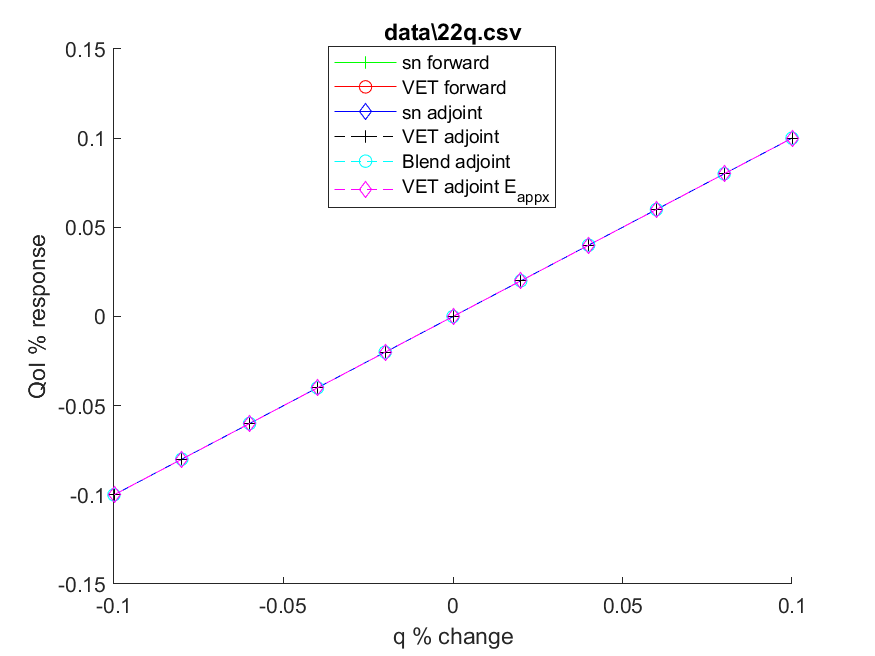
\includegraphics[width=.98\linewidth]{figures2/22qSens.png}
  \label{T1:sfig1}
\end{subfigure}%
\begin{subfigure}{.5\textwidth}
  \centering
  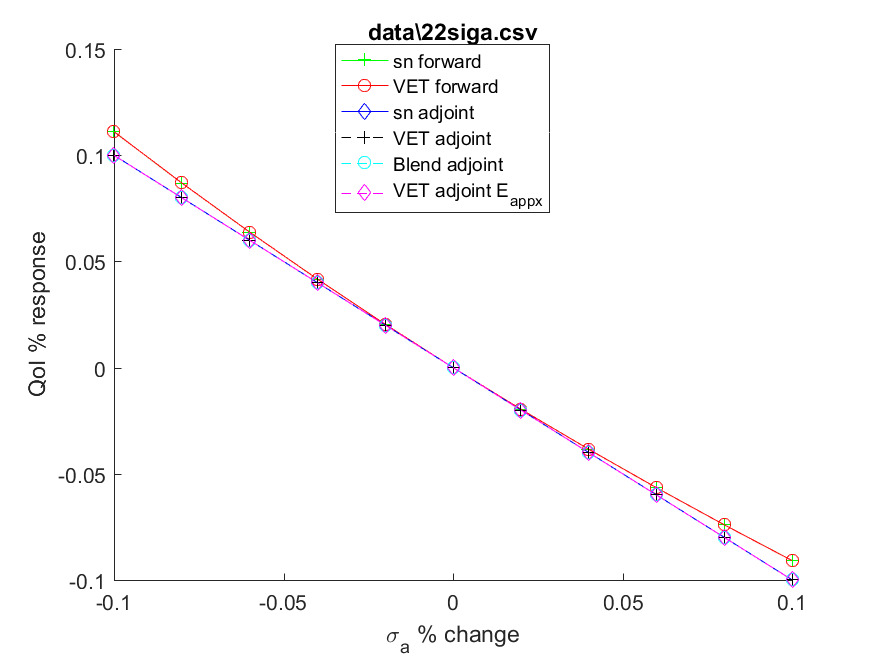
\includegraphics[width=.98\linewidth]{figures2/22sigaSens.png}
  \label{T1:sfig2}
\end{subfigure}
%
\begin{subfigure}{.5\textwidth}
  \centering
  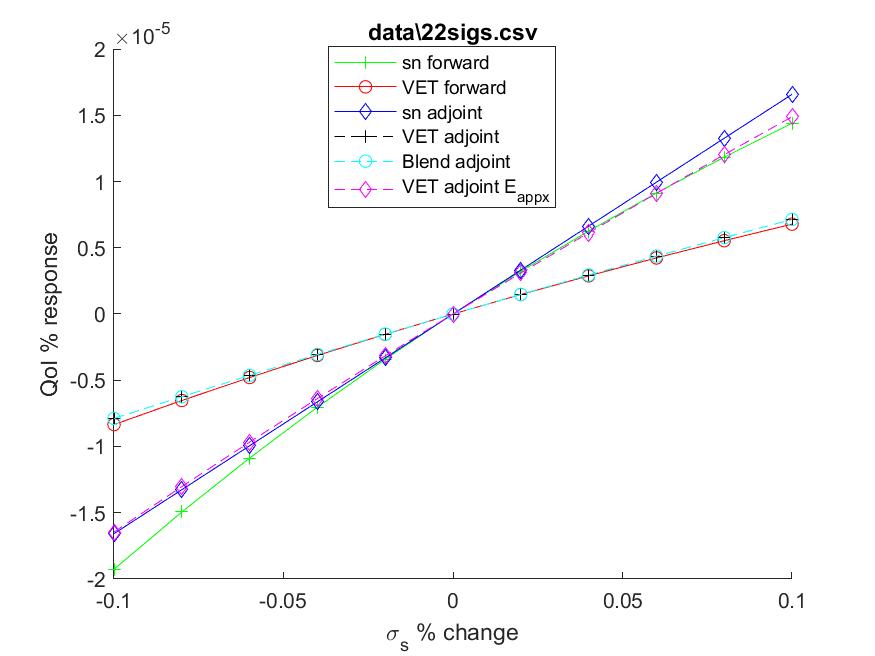
\includegraphics[width=.98\linewidth]{figures2/22sigsSens.png}
  \label{T1:sfig3}
\end{subfigure}%
\begin{subfigure}{.5\textwidth}
  \centering
  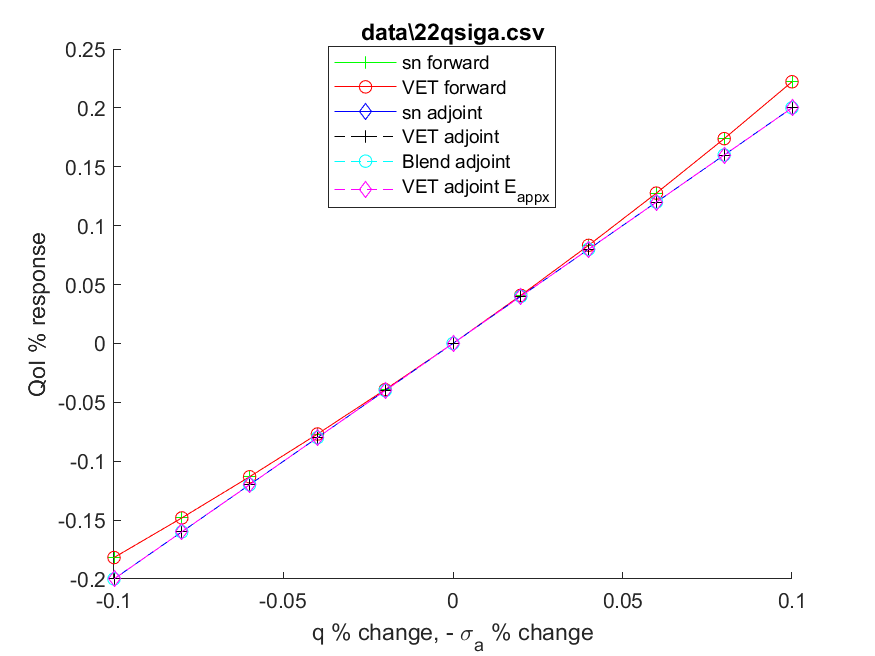
\includegraphics[width=.98\linewidth]{figures2/22qsigaSens.png}
  \label{T1:sfig4}
\end{subfigure}
\caption{\qoi response to various perturbation scenarios for the homogeneous system under various homogeneous perturbations. For the unperturbed system $q=2$, $\sigt=1$, and $\sigs=1$.}
\end{figure}

In both the unperturbed and perturbed state, the Eddington is essentially at the diffusion limit of $\Edd = 1/3 \mathbb{I}$, so the unperturbed Eddington approximation should be a safe assumption to make in this scenario. The results of the $q$ and $\siga$ perturbations seem to support this. For the source perturbations, no first order approximation is needed, so all methods appear to give the same result. The $\siga$ perturbations begin to show the affects of the first order approximation, adjoint methods diverge from the exact forward methods. As would be expected, the system does not show strong sensitivity to $\sigs$ perturbations.

\begin{table}[H]
\label{TableT1}
\centering
  \begin{tabular}{| l | r | r | r | r |}
    \hline
    Method  &  $+10\% q $  & $-10\% \siga $ & $+10\% \sigs $ & $+10\% q,-10\% \siga$ \\ \hline
     SN Fwd 			&0.39998 &0.44419 &5.7577e-05 & 0.88858\\ \hline
     VET Fwd			&0.39998 &0.44428 &2.7131e-05 &0.88868\\ \hline
     SN Adj			&0.39998 &0.39983 &6.6307e-05 &0.79980\\ \hline
     VET Adj 			&0.39998 &0.39988 &2.8534e-05 &0.79986\\ \hline
     Blended 			&0.39998 &0.39988 &2.8534e-05 &0.79986\\ \hline
     VET $\delta \Edd$ 	&0.39998 &0.39983 &5.9537e-05 &0.79981\\ \hline
    \end{tabular}
  \caption{Table of selected results for the homogeneous system under homogeneous perturbations. Values given are absolute $\delta \Edd$. }
\end{table}


%%%%%%%----------------------------------------------------------------------------------------------
\subsection{Homogeneous System, Inhomogeneous Perturbation}
The initial homogeneous unperturbed system is retained from the previous trial. Now the system is subjected to inhomogeneous perturbations. To accomplish this, only the left $3/5$th of the system experiences the perturbation. This creates generates a material boundary which tends to generate perturbations in $\delta E$.

\begin{figure}[H]
\label{Trial2}
\centering
\begin{subfigure}{.5\textwidth}
  \centering
  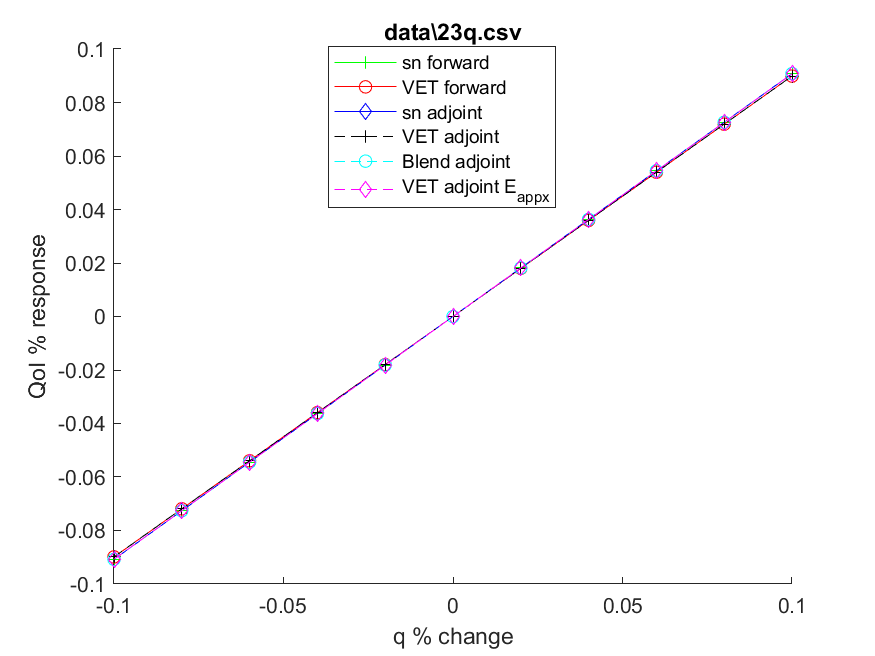
\includegraphics[width=.98\linewidth]{figures2/23qSens.png}
  \label{T2:sfig1}
\end{subfigure}%
\begin{subfigure}{.5\textwidth}
  \centering
  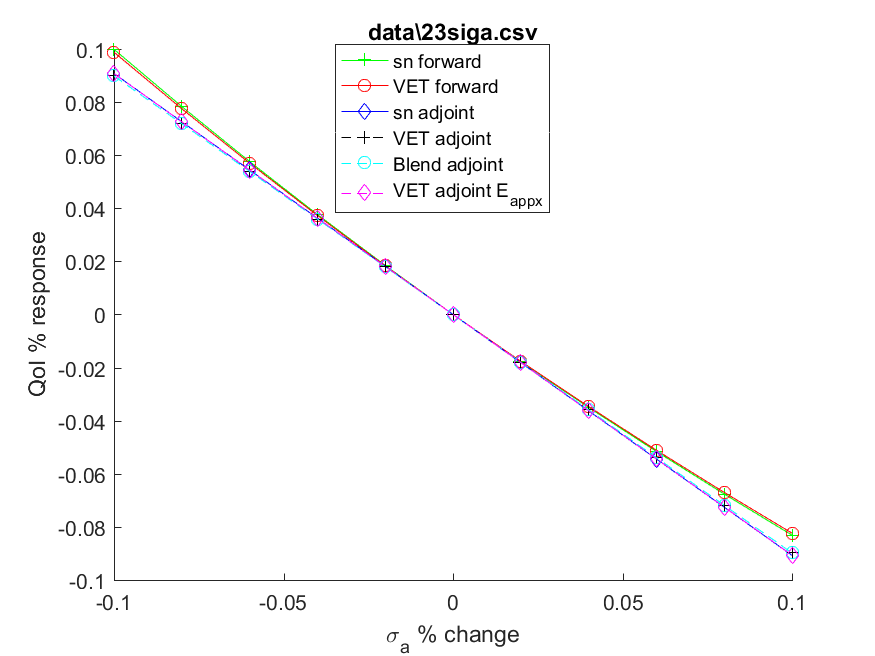
\includegraphics[width=.98\linewidth]{figures2/23sigaSens.png}
  \label{T2:sfig2}
\end{subfigure}
%
\begin{subfigure}{.5\textwidth}
  \centering
  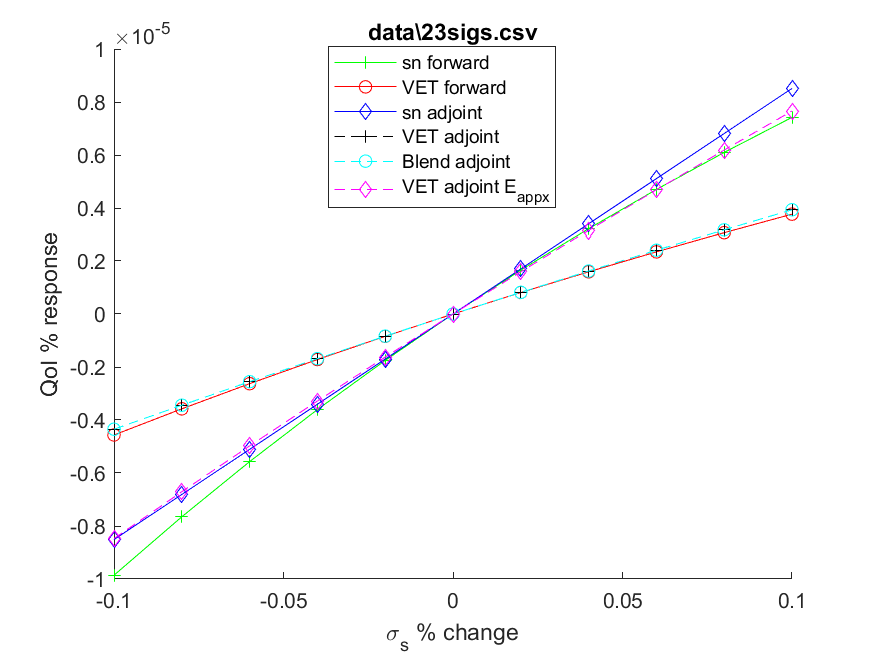
\includegraphics[width=.98\linewidth]{figures2/23sigsSens.png}
  \label{T2:sfig3}
\end{subfigure}%
\begin{subfigure}{.5\textwidth}
  \centering
  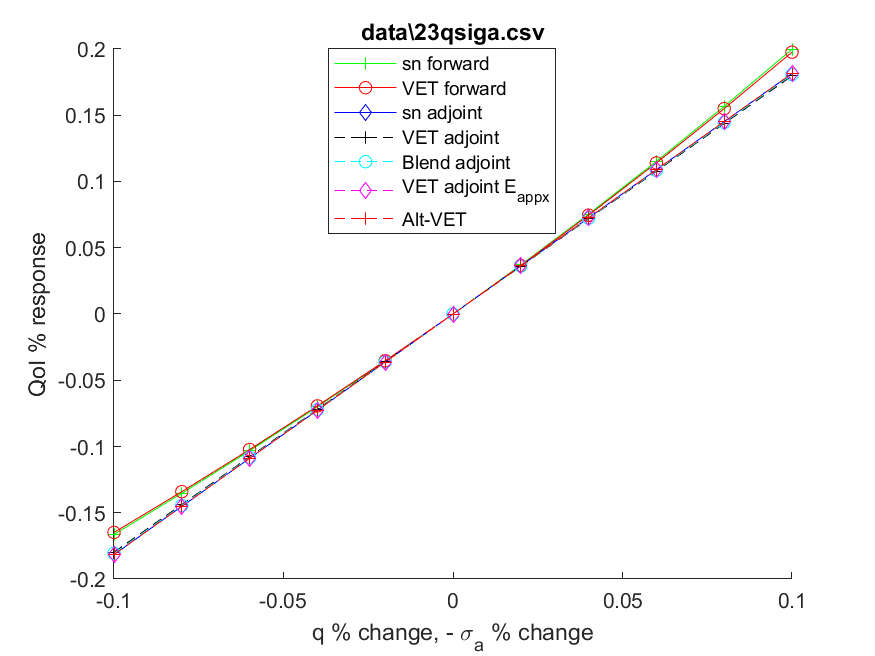
\includegraphics[width=.98\linewidth]{figures2/23qsigaSens.png}
  \label{T2:sfig4}
\end{subfigure}
\caption{\qoi response to various perturbation scenarios for the homogeneous system under various inhomogeneous perturbations. For the unperturbed system $q=2$, $\sigt=1$, and $\sigs=1$.}
\end{figure}

The introduction of the boundary layer in the perturbed state begins to show differentiation in the selected methods. For source perturbations the adjoint methods match their respective forward found values. The blended method matches the SN values for source perturbations and the VET values for cross-section perturbations as designed. The behavior of the blended method with both source and cross-section perturbations shows that it does provide an improvement over the adjoint VET method, however the found value still lies closer to the VET value than the SN adjoint value. The $\delta \Edd$ method shows more promise in this trial, as the addition of the $\delta \Edd$ terms begins to reconcile the VET adjoint method with the more exact SN adjoint. 


\begin{table}[H]
\centering
  \begin{tabular}{| l | r | r | r | r |}
    \hline
    Method  &  $+10\% q $  & $-10\% \siga $ & $+10\% \sigs $ & $+10\% q,-10\% \siga$ \\ \hline
     SN Fwd 			&0.36309 &0.39952 &2.9680e-05 & 0.79915\\ \hline
     VET Fwd			&0.35947 &0.39517 &1.5072e-05 &0.79040\\ \hline
     SN Adj  			&0.36309 &0.36301 &3.4051e-05 &0.72610\\ \hline
     VET Adj 			&0.35947 &0.35941 &1.5733e-05 &0.71888\\ \hline
     Blended 			&0.36309 &0.35941 &1.5733e-05 &0.72250\\ \hline
     VET $\delta \Edd$ 	&0.36287 &0.36290 &3.0640e-05 &0.72586\\ \hline
    \end{tabular}
  \caption{Table of selected results for the homogeneous system under inhomogeneous perturbations. Values given are absolute $\delta \Edd$. }
\end{table}

%%%%%%%----------------------------------------------------------------------------------------------
\subsection{Shielded Incident Flux}
To observe the response to perturbations in the incident flux, a simple shielding system is tested. Flux is incident on the left side of the system. The incident flux passes though a shield of width 1 with $\siga=0.5$ and $\sigs=0.5$. The response is taken on the right side of the shield.


\begin{figure}[H]
\label{Trial3}
\centering
\begin{subfigure}{.5\textwidth}
  \centering
  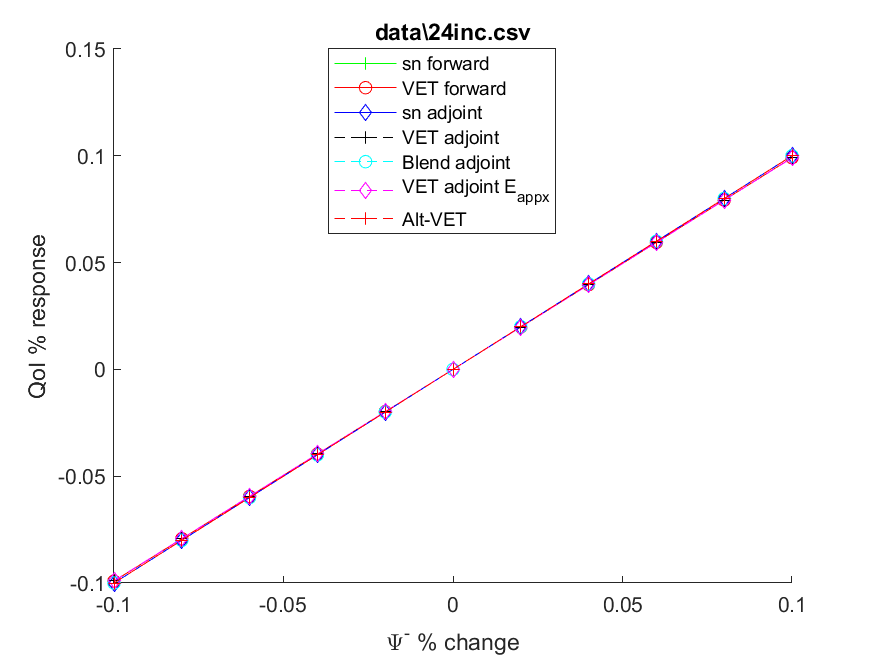
\includegraphics[width=.98\linewidth]{figures2/24incSens.png}
  \label{T3:sfig1}
\end{subfigure}%
\begin{subfigure}{.5\textwidth}
  \centering
  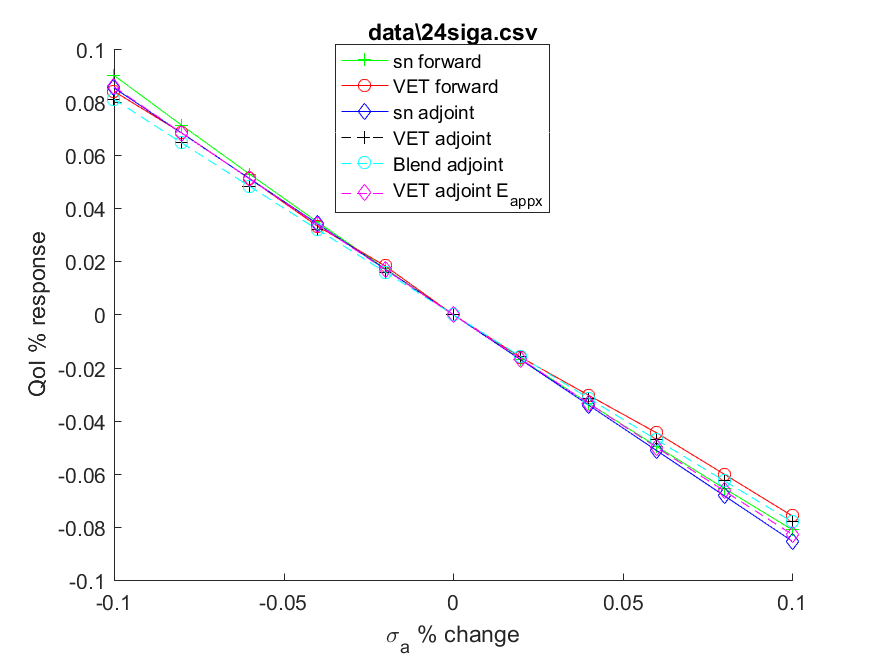
\includegraphics[width=.98\linewidth]{figures2/24sigaSens.png}
  \label{T3:sfig2}
\end{subfigure}
%
\begin{subfigure}{.5\textwidth}
  \centering
  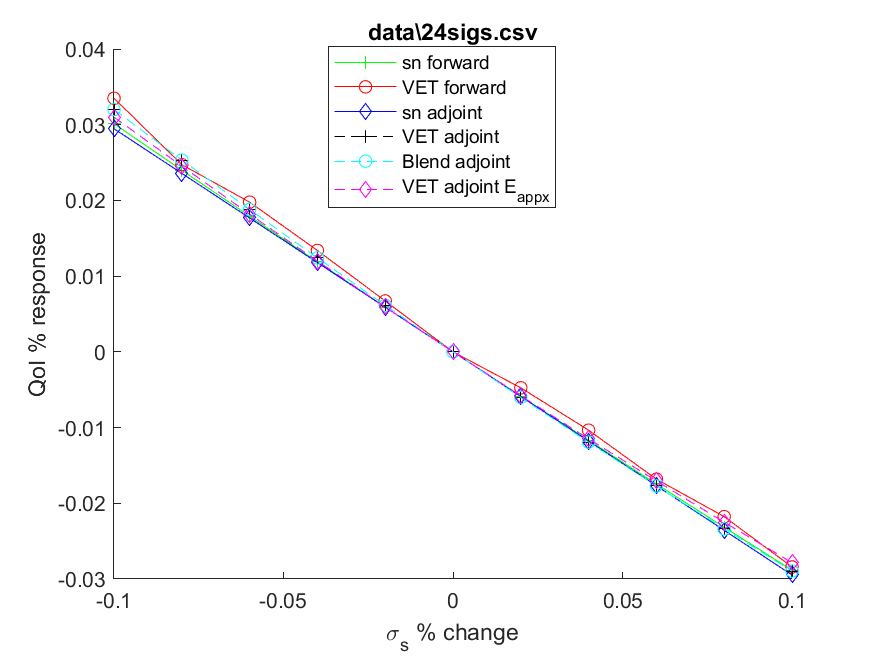
\includegraphics[width=.98\linewidth]{figures2/24sigsSens.png}
  \label{T3:sfig3}
\end{subfigure}%
\begin{subfigure}{.5\textwidth}
  \centering
  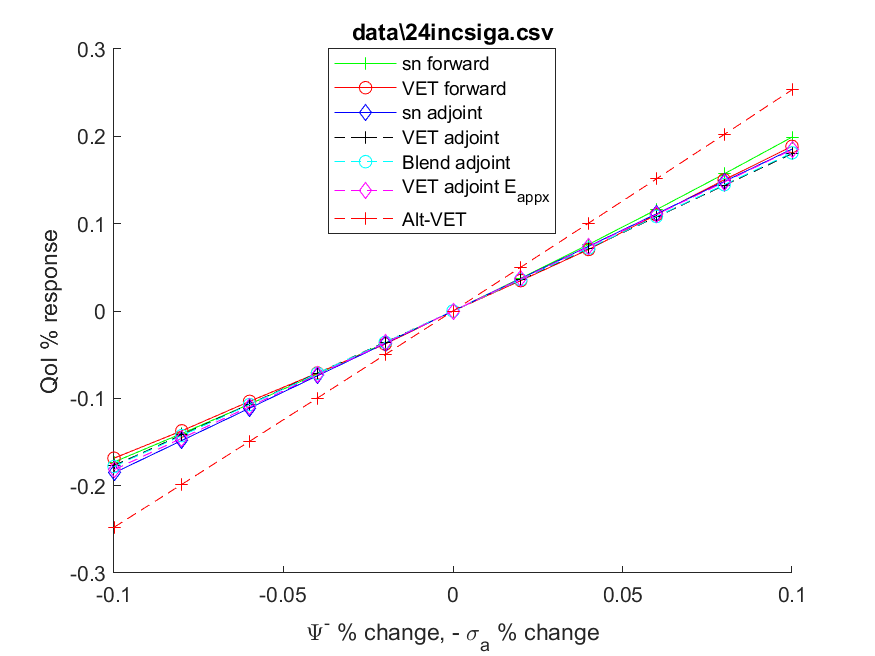
\includegraphics[width=.98\linewidth]{figures2/24incsigaSens.png}
  \label{T3:sfig4}
\end{subfigure}
\caption{\qoi response to various perturbation scenarios for the.}
\end{figure}

Response to perturbation in the incident flux behaves as expected, in that adjoint methods match their respective forward found values. The $\delta E$ approximation method helps approach the SN value in most cases, however when dealing with scattering perturbations, the $\delta E$ method actually results in a $\delta \qoi$ value further from the SN value than the basic VET method. 

\begin{table}[H]
\centering
  \begin{tabular}{| l | r | r | r | r |}
    \hline
    Method  &  $+10\% \psi^- $  & $-10\% \siga $ & $+10\% \sigs $ & $+10\% \psi^-,-10\% \siga$ \\ \hline
     SN Fwd 			&0.023401 &0.021079 &-0.0067476 & 0.046588\\ \hline
     VET Fwd			&0.023181 &0.019670 &-0.0066481 &0.044818\\ \hline
     SN Adj  			&0.023401 &0.019975 &-0.0068956 &0.043376\\ \hline
     VET Adj 			&0.023181 &0.018981 &-0.0067751 &0.042162\\ \hline
     Blended 			&0.023401 &0.018981 &-0.0067751 &0.042381\\ \hline
     VET $\delta \Edd$ 	&0.023181 &0.020070 &-0.0065156 &0.043251\\ \hline
    \end{tabular}
  \caption{Table of selected results for the shielding system under perturbations. Values given are absolute $\delta \Edd$. }
\end{table}

%%%%%%%----------------------------------------------------------------------------------------------
\subsection{Reed Problem}
As a final test, a more varied and complex system is tested. The system is split into 5 regions of unequal length with properties given below. As for perturbations, $\siga$ experiences perturbations in regions 1 and 4, $\sigs$ is perturbed in regions 4 and 5, and $q$ is perturbed in regions 1 and 4. The system has no incident flux.
\begin{equation*}
\begin{split}
&\text{Region 1: } x \in (0,2), \quad \siga=50, \, 			\sigs=0, \, q=50 \, q^\dag=0 \\
&\text{Region 2: } x \in (2,3), \quad \siga=5, \, 			\sigs=0, \, q=0 \, q^\dag=0 \\
&\text{Region 3: } x \in (3,5), \quad \siga \approx 0, \,	\sigs=0, \, q=0 \, q^\dag=0 \\
&\text{Region 4: } x \in (5,6), \quad \siga=0.1, \, 		\sigs=0.9, \, q=1 \, q^\dag=0 \\
&\text{Region 5: } x \in (6,8), \quad \siga=0.1, \, 		\sigs=0.9, \, q=0 \, q^\dag=1 \\
\end{split}
\end{equation*}


\begin{figure}[H]
\label{Trial4}
\centering
\begin{subfigure}{.5\textwidth}
  \centering
  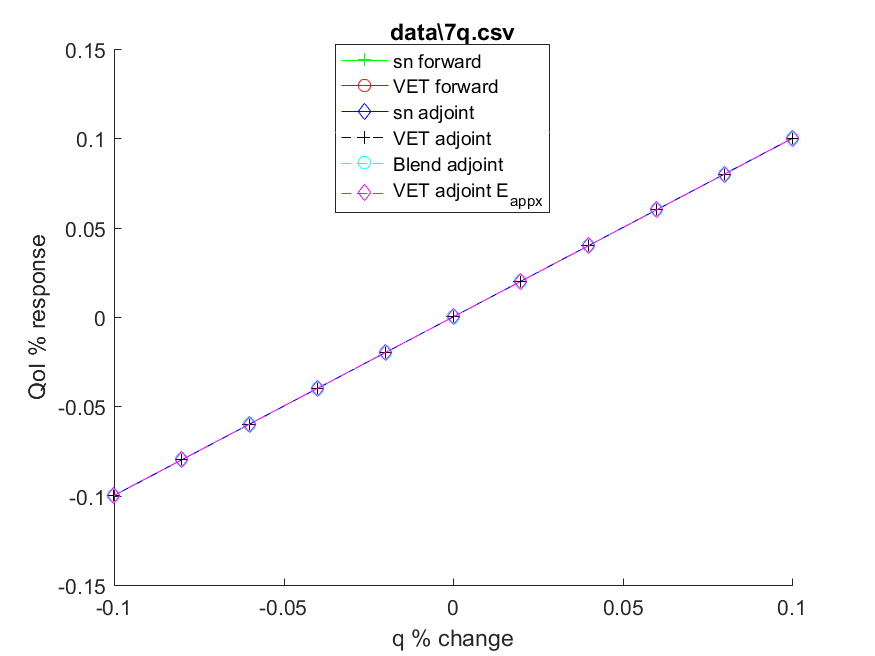
\includegraphics[width=.98\linewidth]{figures2/7qSens.png}
  \label{T4:sfig1}
\end{subfigure}%
\begin{subfigure}{.5\textwidth}
  \centering
  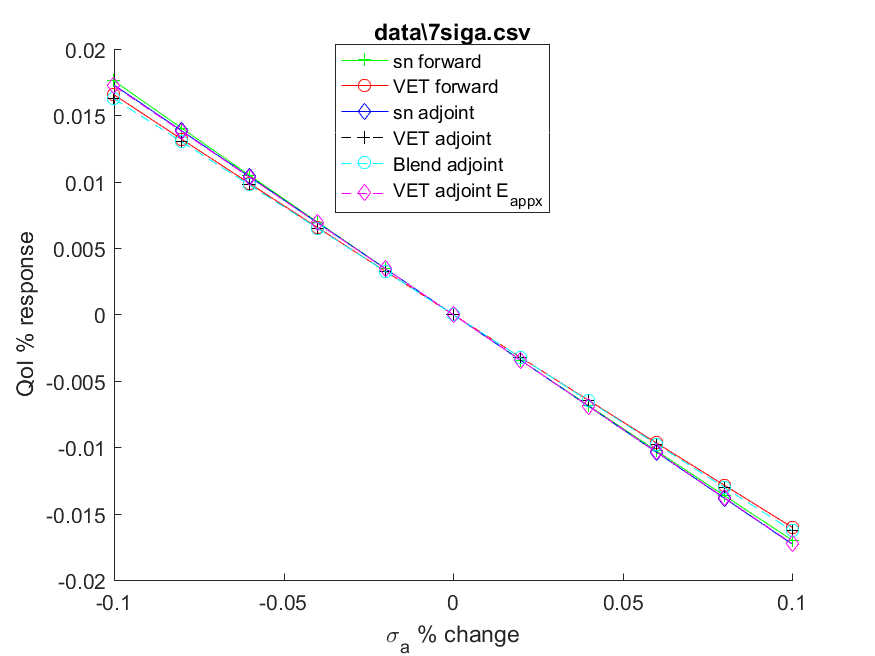
\includegraphics[width=.98\linewidth]{figures2/7sigaSens.png}
  \label{T4:sfig2}
\end{subfigure}
%
\begin{subfigure}{.5\textwidth}
  \centering
  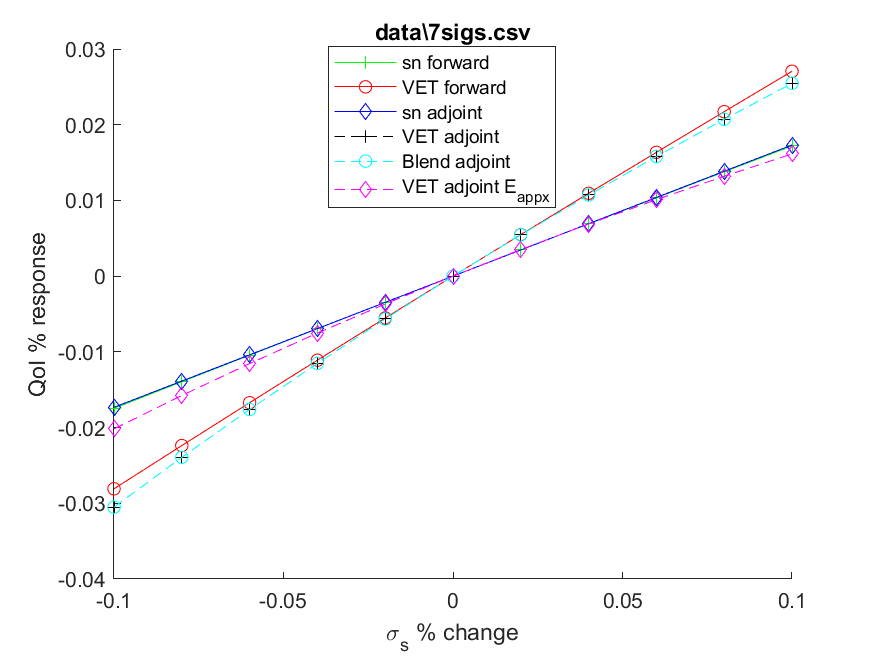
\includegraphics[width=.98\linewidth]{figures2/7sigsSens.png}
  \label{T4:sfig3}
\end{subfigure}%
\begin{subfigure}{.5\textwidth}
  \centering
  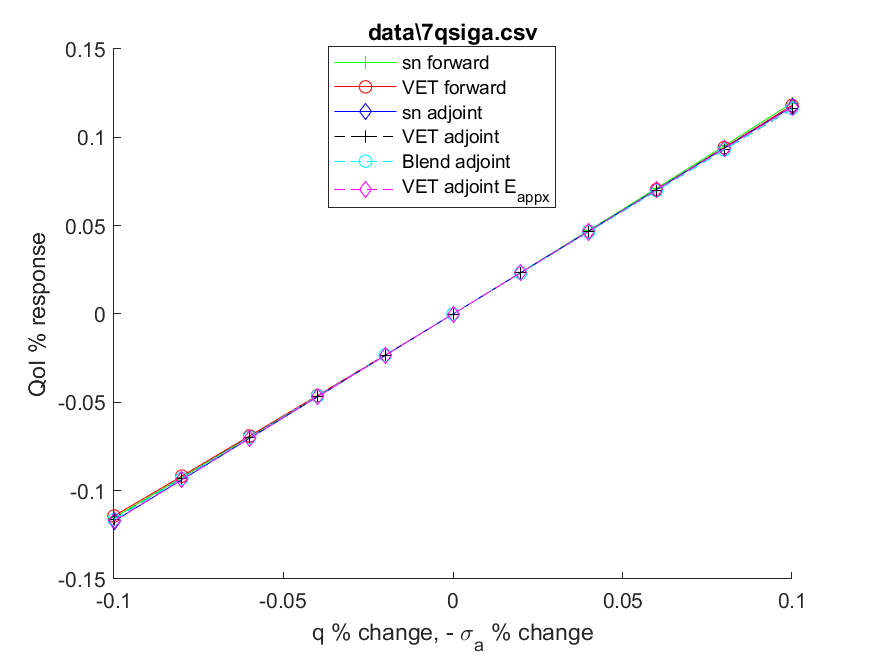
\includegraphics[width=.98\linewidth]{figures2/7qsigaSens.png}
  \label{T4:sfig4}
\end{subfigure}
\caption{\qoi response to various perturbation scenarios for the Reed Problem.}
\end{figure}

The effect of scattering perturbations is more pronounced in the Reed problem, along with the error between the SN and VET derived methods. The $\Delta \Edd$ approximation method proves quite valuable in this problem however, and moves the response much closer to the SN adjoint found sensitivity for cross-section perturbations. 

\begin{table}[H]
\centering
  \begin{tabular}{| l | r | r | r | r |}
    \hline
    Method  &  $+10\% q $  & $-10\% \siga $ & $+10\% \sigs $ & $+10\% q,-10\% \siga$ \\ \hline
     SN Fwd 			&0.17580 &0.030945 &0.030235 & 0.20984\\ \hline
     VET Fwd 			&0.17561 &0.029105 &0.047568 &0.20763\\ \hline
     SN Adj 			&0.17580 &0.030401 &0.030450 &0.20620\\ \hline
     VET Adj 			&0.17561 &0.028580 &0.044778 &0.20419\\ \hline
     Blended 			&0.17580 &0.028580 &0.044778 &0.20438\\ \hline
     VET $\delta \Edd$ 	&0.17561 &0.030291 &0.028388 &0.20590\\ \hline
    \end{tabular}
  \caption{Table of selected results for the Reed system under perturbations. Values given are absolute $\delta \Edd$. }
\end{table}

\chapter{\uppercase {Conclusion and looking ahead}}

For the systems tested, the VET method shows promise for use in sensitivity calculations. For the majority of the trials the error between the VET and SN adjoint sensitivities was $<10\%$ of the SN sensitivity, and $<1\%$ of the unperturbed QoI. The blended method demonstrated an approach to increase the accuracy, particularly for source perturbations, at the cost of an additional SN solve to obtain $\phi$. The $\delta \Edd$ approximation approach was even more accurate in most cases, but requires at least 1 extra SN solve for each perturbed system property, making it viable in scenarios where many perturbation scenarios must be tested. 

Scattering perturbations showed possibly the most interesting behavior. The deviation of the VET and SN methods is stronger (relative to the SN sensitivity) in most of the test case when $\sigs$ is perturbed. Additionally, the shielding system presented a scenario where the $\delta \Edd$ approach appeared to introduce more error. Unfortunately, the testing of heavy scatting systems in one spacial dimension can be a bit limited. In a two or three dimensions, the ability for particles to scatter around objects exists in general, while this is not present in one dimension. Expanding the discussed concepts to higher spacial dimensions would be a worthwhile next step, particularly in observing the effects of scattering on the VET method.


\section{Looking towards time dependence}
While out of scope for this writing, a major goal of this method is the application towards time-dependent systems. As such, it is worth taking a brief look at how the VET formulation would look in a time dependent system. As with the steady state, the starting point is the one-group transport equation, now with the time derivative factor.
\begin{equation}
\label{Trans1GTE}
\frac{1}{v} \frac{\partial}{\partial t} \psi(\vr,\vO,t)+ \vO \cdot \grad \psi(\vr,\vO,t) + \sigt(\vr) \psi(\vr,\vO,t) = \frac{1}{4 \pi} \sigs(\vr) \phi(\vr) + q(\vr,\vO,t), \quad \forall \vr \in V,t \geq 0
\end{equation}
\begin{equation}
\label{Trans1GTE_bc}
\psi(\vr,\vO,t) = \psi^{\text{inc}}(\vr,\vO,t) \quad \vr \in \partial V^{-} = \{ \vr \in \partial V, \text{ s.t. }, \vO \cdot \vec{n}(\vr) < 0\}
\end{equation}
\begin{equation}
\label{Trans1GTE_t0}
\psi(\vr,\vO,0) = \psi_0(\vr,\vO)
\end{equation}
The zero-th and first angular moments are taken of the time dependent system. The Eddington Tensor is used in the 1st order equation.
\begin{subequations}
%
\begin{equation}
\label{0amTrans}
\frac{1}{v} \frac{\partial}{\partial t}\phi + \div \vec{J} + (\siga) \phi = \scalSource \,,
\end{equation}
%
\begin{equation}
\label{1amTrans}
\frac{1}{v} \frac{\partial}{\partial t}\vec{J}  + \div \left( \Edd \phi \right) + \sigt \vec{J} = 0 \,.
\end{equation}
%
\end{subequations}
The moments are then combined in the same fashion used in the steady-state case
\begin{equation}
\label{VETTrans}
\frac{1}{v} \frac{\partial}{\partial t}\phi - \div \left( \frac{1}{v \sigt} \frac{\partial}{\partial t}\vec{J} \right)   - \div \left( \frac{1}{\sigt} \div \left( \Edd \phi \right) \right)  + (\siga) \phi = \scalSource.
\end{equation}
\iwh{Not sure on the exact next step to take. The second term is the ugly one. I can define the residual 
\begin{equation}
f=- \div \left( \frac{1}{\sigt} \div \left( \Edd \phi \right) \right)  + (\siga) \phi - \scalSource
\end{equation}
which is the steady state equation, and muse about how that term must be dealt with accurately to produce time evolution. 
Doing sensitivity we want an operator $A \phi = b$ which the above isn't exactly due to the $\vec{J}$. In addition to $\Edd$ is is reasonable to store some vector value like $\vec{g}=\frac{\vec{J}}{\phi}$? That way there is a well defined $A$ operator to perform the adjoint process on.}

%The next line is the format for inserting new sections.
%Replace the name "newsection"  with the name of your
%new section file.
%\include{data/newsection}


%\bibliography{IanProp} 
%\bibliographystyle{ieeetr}

%fix spacing in bibliography, if any...
%%%%%%%%%%%%%%%%%%%%%%%%%%%%%%%%%%%%%%%%%%%%%%%%%%%%%%%%%%%%%
\let\oldbibitem\bibitem
\renewcommand{\bibitem}{\setlength{\itemsep}{0pt}\oldbibitem}
%%%%%%%%%%%%%%%%%%%%%%%%%%%%%%%%%%%%%%%%%%%%%%%%%%%%%%%%%%%%%%%
%The bibliography style declared is the IEEE format. If
%you require a different style, see the document
%bibstyles.pdf included in this package. This file,
%hosted by the University of Vienna, shows several
%bibliography styles and examples of in-text citation
%and a references page.
\bibliographystyle{ieeetr}

\phantomsection
\addcontentsline{toc}{chapter}{REFERENCES}

\renewcommand{\bibname}{{\normalsize\rm REFERENCES}}

%This file is a .bib database that contains the sources.
%This removes the dependency on the previous file
%bibliography.tex.
\bibliography{IanProp}




%This next line includes appendices. The file
%appendix.tex contains commands pointing to
%the appendix files; be sure to change these
%pointers if you end up changing the filenames.
%Leave this commented if you will not need
%appendix material.
%%%%%%%%%%%%%%%%%%%%%%%%%%%%%%%%%%%%%%%%%%%%%%%%%%%%
%
%  New template code for TAMU Theses and Dissertations starting Fall 2016.  
%
%
%  Author: Sean Zachary Roberson
%  Version 3.17.06
%  Last Updated: 6/15/2017
%
%%%%%%%%%%%%%%%%%%%%%%%%%%%%%%%%%%%%%%%%%%%%%%%%%%%

\begin{appendices}
\titleformat{\chapter}{\centering\normalsize}{APPENDIX \thechapter}{0em}{\vskip .5\baselineskip\centering}
\renewcommand{\appendixname}{APPENDIX}

%%%%%%%%%%%%%%%%%%%%%%%%%%%%%%%%%%%%%%%%%%%%%%%%%%%
%
%  New template code for TAMU Theses and Dissertations starting Fall 2016.
%
%
%  Author: Sean Zachary Roberson 
%	 Version 3.16.09
%  Last updated 9/12/2016
%
%%%%%%%%%%%%%%%%%%%%%%%%%%%%%%%%%%%%%%%%%%%%%%%%%%%

%%%%%%%%%%%%%%%%%%%%%%%%%%%%%%%%%%%%%%%%%%%%%%%%%%%%%%%%%%%%%%%%%%%%%%
%%                           APPENDIX A 
%%%%%%%%%%%%%%%%%%%%%%%%%%%%%%%%%%%%%%%%%%%%%%%%%%%%%%%%%%%%%%%%%%%%%

\phantomsection

\chapter{\uppercase{First Appendix}}

Text for the Appendix follows.

\begin{figure}[h]
\centering
%\includegraphics[scale=.50]{figures/Penguins.jpg}
\caption{TAMU figure}
\label{fig:tamu-fig5}
\end{figure}

%%%%%%%%%%%%%%%%%%%%%%%%%%%%%%%%%%%%%%%%%%%%%%%%%%%
%
%  New template code for TAMU Theses and Dissertations starting Fall 2016.
%
%
%  Author: Sean Zachary Roberson 
%	 Version 3.16.09 
%  Last updated 9/12/2016
%
%%%%%%%%%%%%%%%%%%%%%%%%%%%%%%%%%%%%%%%%%%%%%%%%%%%

%%%%%%%%%%%%%%%%%%%%%%%%%%%%%%%%%%%%%%%%%%%%%%%%%%%%%%%%%%%%%%%%%%%%%%
%%                           APPENDIX B
%%%%%%%%%%%%%%%%%%%%%%%%%%%%%%%%%%%%%%%%%%%%%%%%%%%%%%%%%%%%%%%%%%%%%

\chapter{\uppercase {A Second Appendix Whose Title Is Much Longer Than The First}}

Text for the Appendix follows.

\begin{figure}[h]
\centering
%\includegraphics[scale=.50]{figures/Penguins.jpg}
\caption{Another TAMU figure.}
\label{fig:tamu-fig6}
\end{figure}

\section{Appendix Section}

\section{Second Appendix Section}


\pagebreak{}

\end{appendices}


\end{document}
